\chapter{ابزارها و کتابخانه‌ها}

در این فصل، نگاهی به تمام ابزار‌ها و کتابخانه‌‌های مورد استفاده پروژه می‌اندازیم. دانستن نحوه معماری و کارکرد این ابزارها، برای درک فصل طراحی و پیاده‌سازی پروژه، ضروری است.

\section{\lr{ROS}}
\lr{ROS}\LTRfootnote{\lr{Robot Operating System}}، مجموعه‌ای از کتابخانه‌های نرم‌افزاری و ابزارها است که در زمینه پیاده‌سازی ربات‌ها فعالیت ‌می‌کنند. \lr{ROS} یک بسته توسعه نرم‌افزار\LTRfootnote{\lr{Software Development Kit (SDK)}} ربات متن‌باز\LTRfootnote{\lr{Open Source}} است. این نرم‌افزار،‌ یک سکوی نرم‌افزاری را در دسترس توسعه‌گران صنعت رباتیک گذاشته است تا به تحقیقات، نمونه‌سازی‌ و گسترش علم رباتیک سرعت بخشد. 
\lr{ROS} بیش از ۱۰ سال است که در صنعت رباتیک، توسط میلیون‌ها توسعه‌گر در حال استفاده است. این نرم‌افزار، در اکثر سیستم‌ عامل‌ها و سیستم‌های نهفته\LTRfootnote{\lr{Embedded Systems}} قابل توسعه است، و در حوزه‌های پردازش بلادرنگ نیز نقشی اساسی دارد \cite{doi:10.1126/scirobotics.abm6074}.

\subsection{اکوسیستم}
برخلاف اسم ‌آن، \lr{ROS} یک سیستم‌ عامل نیست و همانطور که ذکر شد، یک بسته توسعه نرم‌افزار ربات است. اکوسیستم این بسته نرم‌افزاری به شکل زیر است:

\begin{figure}[h!]
    \centering
    
\includegraphics[width=1\linewidth]{figures/ROS_Ecosystem.png}
    \caption{تصویری از اجزای \lr{ROS} \cite{ROS:2023}}
    \label{fig:ROS_ecosystem}
\end{figure}

همانطور که مشاهده ‌می‌کنیم، اکوسیستم نرم‌افزار \lr{ROS} از چهار بخش اساسی تشکیل شده است:
\begin{enumerate}
    \item \textbf{لوله‌کشی}\LTRfootnote{\lr{Plumbing}}: در اصل، \lr{ROS} یک سیستم انتقال پیام فراهم می‌کند که اغلب به عنوان "میان‌افزار\LTRfootnote{\lr{Middleware}}" یا "لوله‌کشی" شناخته می‌شود. ارتباط اولین نیازی است که هنگام پیاده‌سازی یک برنامه رباتیک جدید یا به طور کلی هر سیستم نرم‌افزاری که با سخت‌افزار تعامل خواهد داشت، به وجود می‌آید. سیستم پیام‌دهی محبوب و تست‌شده‌ \lr{ROS}، باعث صرفه جویی در زمانی می‌شود که برای مدیریت جزئیات مربوط به ارتباط بین گره‌های\LTRfootnote{\lr{Nodes}} توزیع‌شده،‌ صرف شده است (از طریق یک الگوی انتشار/اشتراک ناشناس\LTRfootnote{\lr{Anonymous Publish/Subscribe Patterns}}). این رویکرد به شما کمک می‌کند تا شیوه‌های خوبی را در توسعه نرم‌افزار‌های خود رعایت کنید، که شامل جدا کردن ایرادها، جداسازی نیازمندی‌ها و رابط‌هایی\LTRfootnote{\lr{Interface}} واضح می‌شود. استفاده از \lr{ROS} منجر به ایجاد سیستم‌هایی می‌شود که آنها را آسان‌تر برای نگهداری، مشارکت در توسعه، و استفاده مجدد می‌کند.
    
    در طی این مسیر، می‌توان از تجربیات جامعه گسترده‌ای که به ایجاد استانداردهای پیام \lr{ROS} منجر شده است، بهره برد. این استانداردها برای تعامل با همه چیز از سنجش فاصله لیزری و دوربین‌ها تا الگوریتم‌های موقعیت‌یابی و رابط‌های کاربری استفاده می‌شوند \cite{ROS:2023}.
    \item ابزار: پیاده‌سازی برنامه‌های رباتیک چالش‌برانگیز است. شما با تمام مشکلات هر تلاش توسعه نرم‌افزاری مواجه می‌شوید و علاوه بر آن، نیاز به ارتباط ناهمگام\LTRfootnote{\lr{Asynchronous Interaction}} با دنیای فیزیکی از طریق حسگرها و اعمال‌کننده‌ها هم به لیست مشکلات اضافه می‌شود. برای ساختن برنامه‌ها به صورت کارآمد، به ابزارهای توسعه‌دهنده خوبی نیاز است. \lr{ROS} این ابزارها را دارد که شامل ابزارهایی مانند راه‌اندازی\LTRfootnote{\lr{Launch}}، خودکاوی\LTRfootnote{\lr{Introspection}}، اشکال‌زدایی\LTRfootnote{\lr{Debugging}}، بصری‌سازی\LTRfootnote{\lr{Visualization}}، کشیدن نمودار، ثبت اتفاقات\LTRfootnote{\lr{Logging}} و پخش\LTRfootnote{\lr{Playback}} می‌شوند. این ابزارها به پیشرفت تیم‌های توسعه، شتاب می‌دهند و می‌توانند همراه محصول عرضه ‌شده قرار گیرند \cite{ROS:2023}.

    \item قابلیت‌ها: جامعه‌ی \lr{ROS} یک مجموعه‌ی نرم‌افزارهای رباتیک است. اگر نیاز به یک درایور برای دستگاه موقعیت‌یاب دارید، یا به یک کنترل کننده‌ی حرکت و تعادل برای ربات چهارپا، یا یک سیستم نقشه‌برداری برای ربات متحرکتان، \lr{ROS} ابزاری برای شما دارد. از درایورها تا الگوریتم‌ها و رابط‌های کاربری، \lr{ROS} اجزای اصلی را فراهم می‌کند که به شما اجازه می‌دهد تا بر روی برنامه‌ی خود تمرکز کنید. هدف پروژه‌ی \lr{ROS}، ارتقاء همیشگی استانداردهای رایج و از این راه کاهش مانع در توسعه برنامه‌های رباتیک است. هر کسی که یک ایده خوب برای یک ربات مفید (یا سرگرم‌کننده، یا جالب) دارد، باید بتواند آن ایده را بدون نیاز به درک تمامی اجزای نرم‌افزاری و سخت‌افزاری مرتبط آن، به واقعیت تبدیل کند \cite{ROS:2023}.

    \item جامعه: جامعه \lr{ROS} وسیع، متنوع و جهانی است. از آدم‌های علاقه‌مند عادی تا دانشجویان، حتی شرکت‌های بین‌المللی و دولت‌ها نیز از ‌\lr{ROS} برای توسعه تکنولوژی رباتیک استفاده می‌کنند.
\end{enumerate}

\subsection{نسخه‌ها}

نرم‌افزار \lr{ROS}، دو نسخه اصلی دارد که \lr{ROS1} و \lr{ROS2} نام دارند. امروزه بیشتر شرکت‌ها از نسخه \lr{ROS2} استفاده می‌کنند زیرا از نظر زیرساخت شبکه‌ای، امنیت و قابلیت‌های توسعه با استانداردهای امروزه، پیشرفته‌تر است. 
\begin{figure}[h!]
    \centering
    \includegraphics[width=0.8\linewidth]{figures/ROS1_ROS2_comparison.png}
    \caption{تفاوت قابلیت‌های \lr{ROS2} نسبت به \lr{ROS1}\cite{doi:10.1126/scirobotics.abm6074}}
    \label{fig:ROS1_ROS2_comparison}
\end{figure}

هر کدام از نسخه‌های \lr{ROS}، توزیع‌هایی\LTRfootnote{\lr{ROS Distributions}} را در اختیار توسعه‌دهندگان قرار داده‌اند. از آنجایی که در این پژوهش نیز از نسخه جدید‌تر \lr{ROS2} استفاده شده است. در \cref{fig:ROS2_Distributions} می‌توانیم چهار توزیع اصلی مورد استفاده توسعه‌دهندگان رباتیک را مشاهده کنیم. در این پژوهش، از توزیع \lr{ROS2 Humble} استفاده شده است که نسخه پایدار و بروز سال ۲۰۲۳ به حساب می‌آید.
\\
\\
\\
\begin{figure}[h]
    \centering
    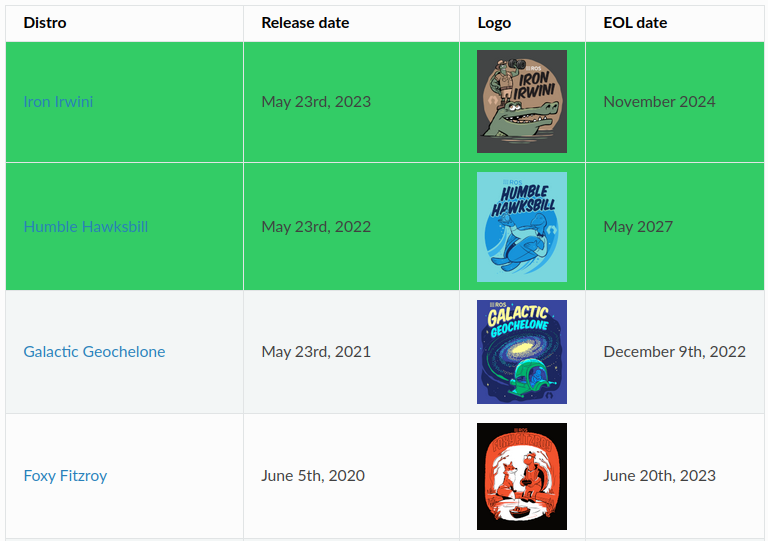
\includegraphics[width=0.8\linewidth]{figures/ROS2_Distributions.png}
    \caption{چهار توزیع اصلی \lr{ROS2}}
    \label{fig:ROS2_Distributions}
\end{figure}

\subsection{معماری بسته توسعه نرم‌افزار \lr{ROS2}}
هر نرم‌افزار توسعه شده توسط \lr{ROS2}، از چند اجزای اصلی تشکیل شده است که در ادامه با آنها آشنا خواهیم شد.

\subsubsection{گراف \lr{ROS2}}
گراف \lr{ROS2}\LTRfootnote{\lr{ROS2 Graph}}، شبکه‌ای از عناصر \lr{ROS2} است که در هم‌زمان در کنار یکدیگر داده‌ها را پردازش می‌کنند. این گراف شامل تمامی اتصالات شبکه‌ی داده‌ای و عناصر قابل اجرا است. 

\subsubsection{گره \lr{ROS2}}
گره \lr{ROS2}\LTRfootnote{\lr{ROS2 Node}}، یک شرکت‌کننده در گراف \lr{ROS2} که از یک کتابخانه کلاینت\LTRfootnote{\lr{Client Library}}، برای ارتباط با سایر گره‌ها استفاده می‌کند. گره‌ها می‌توانند با سایر گره‌ها در داخل همان فرایند، در یک فرایند متفاوت، یا در ماشین متفاوتی ارتباط برقرار می‌کنند. معمولا، گره‌ها واحد محاسباتی در یک گراف  \lr{ROS} هستند؛ هر گره باید یک کار منطقی انجام دهد.

گره‌ها می‌توانند داده‌های خود را به مبحثی\LTRfootnote{\lr{Topic}} انتشار کنند\LTRfootnote{\lr{Publish}} تا بقیه گره‌ها استفاده کنند، یا در موضوعی اشتراک داشته باشند\LTRfootnote{\lr{Subscribe}} و اطلاعات دریافت کنند. آن‌ها می‌توانند به عنوان یک سرویس‌ کلاینت\LTRfootnote{\lr{Service Client}} عمل کنند و محاسبات خود را بر عهده گره دیگری قرار دهند، یا خودشان یک سرویس سرور\LTRfootnote{\lr{Service Server}} باشند و کار محاسبات بقیه گره‌ها را بر عهده بگیرند. برای محاسباتی که طولانی هستند، این گره‌ها می‌توانند یک کلاینت عمل\LTRfootnote{\lr{Action Client}} باشند یا یک سرور عمل‌\LTRfootnote{\lr{Action Server}} باشند. گره‌ها می‌توانند پارامتر‌های\LTRfootnote{\lr{Parameters}} قابل تنظیمی داشته باشند که در حین اجرا توسط بقیه گره‌ها تنظیم شوند.
\begin{definition}
گره یک واحد سازمان‌دهنده مهم است که به کاربر امکان تفکر درباره یک سیستم پیچیده را می‌دهد \cite{doi:10.1126/scirobotics.abm6074}.
\end{definition}

\begin{figure}[h!]
    \centering
    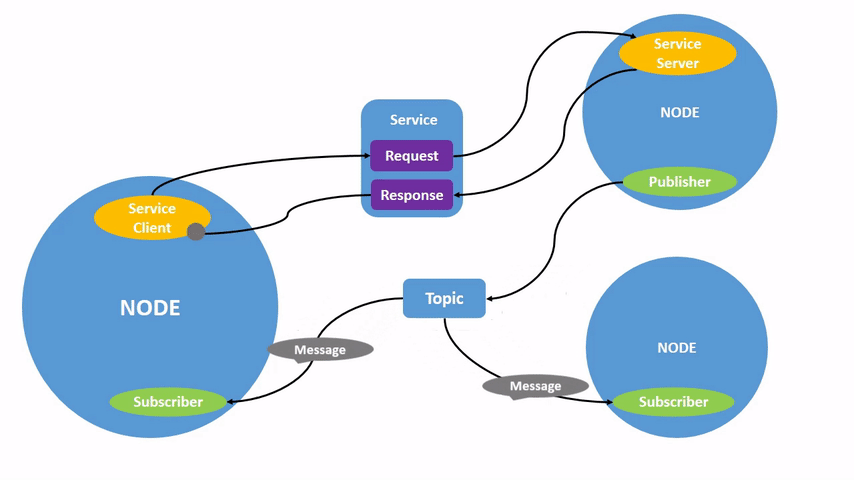
\includegraphics[width=0.75\linewidth]{figures/ROS2_Node_Graph.png}
    \caption{یک گراف ‌\lr{ROS2} ساده \cite{ROS2:Humble_Documentation}}
    \label{fig:ROS2_Node_Graph}
\end{figure}

\subsubsection{رابط‌ها}
تمامی برنامه‌ها و گره‌های توسعه شده تحت \lr{ROS}، از  سه نوع الگوی اصلی برای ارتباط استفاده می‌کنند:
\begin{itemize}
    \item \textbf{‌مبحث‌ها}: الگوی رایج‌تری که کاربران با آن تعامل می‌کنند، مبحث‌ها هستند که یک چارچوب انتقال پیام ناهمگام هستند. کاربران برای ارسال یا دریافت پیام از مبحث‌ها، بایستی از روش انتشار/اشتراک استفاده کنند. ‌\lr{ROS2} تمرکز خود را بر روی استفاده از پیام‌رسانی ناهمگام برای سازماندهی یک سیستم با رابطه‌های قوی متناظر گذاشته است و این کار را با سازماندهی نقاط پایانی\LTRfootnote{\lr{Endpoints}} در یک گراف محاسباتی تخت مفهوم گره انجام می‌دهد. معماری انتشار-اشتراک ناشناس، ارتباطات چند به چند\LTRfootnote{\lr{Many to Many}} را امکان‌پذیر می‌کند. یک توسعه‌دهنده می‌تواند با ایجاد یک اشتراک به یک مبحث، تمام پیام‌های عبوری از این مبحث را بدون اعمال تغییری در عملکرد آن، مشاهده کند \cite{doi:10.1126/scirobotics.abm6074}.
    \item \textbf{سرویس‌ها}: ارتباط ناهمگان همیشه بهترین ابزار نیست. \lr{ROS2} یک الگوی ارتباطی درخواست-پاسخ\LTRfootnote{\lr{Request-Response}}، به نام سرویس‌ها را نیز فراهم می‌کند. ارتباط درخواست-پاسخ تخصیص داده بین یک جفت درخواست و پاسخ را آسان می‌کند. به طور منحصر به فرد، \lr{ROS2} به یک پردازش‌گر سرویس اجازه می‌دهد که در طول یک فراخوانی به آن، مسدود\LTRfootnote{\lr{Blocking}} نشود که یعنی در‌خواست‌ها و پاسخ‌های دیگر هم بتوانند پردازش شوند و منتظر نمانند. سرویس‌ها نیز تحت گره‌ها سازماندهی می‌شوند \cite{doi:10.1126/scirobotics.abm6074}. 
    \item \textbf{اعمال}: اعمال، الگوی ارتباط منحصر‌ به‌ فرد \lr{ROS2} است. اعمال هدف محور هستند و ارتباط‌هایی ناهمگام با الگوی درخواست، پاسخ، و بازخورد دوره‌ای با قابلیت لغو هستند. این الگوی ارتباطی، در وظایف طولانی مانند مسیریابی خودکار یا مدیریت خودکار استفاده می‌شود، اگرچه کاربردهای دیگری هم دارد. مشابه سرویس‌ها، عمل‌ها بدون مسدود کردن هستند و تحت گره سازماندهی می‌شوند \cite{doi:10.1126/scirobotics.abm6074}.
\end{itemize}

\begin{figure}[h!]
    \centering
    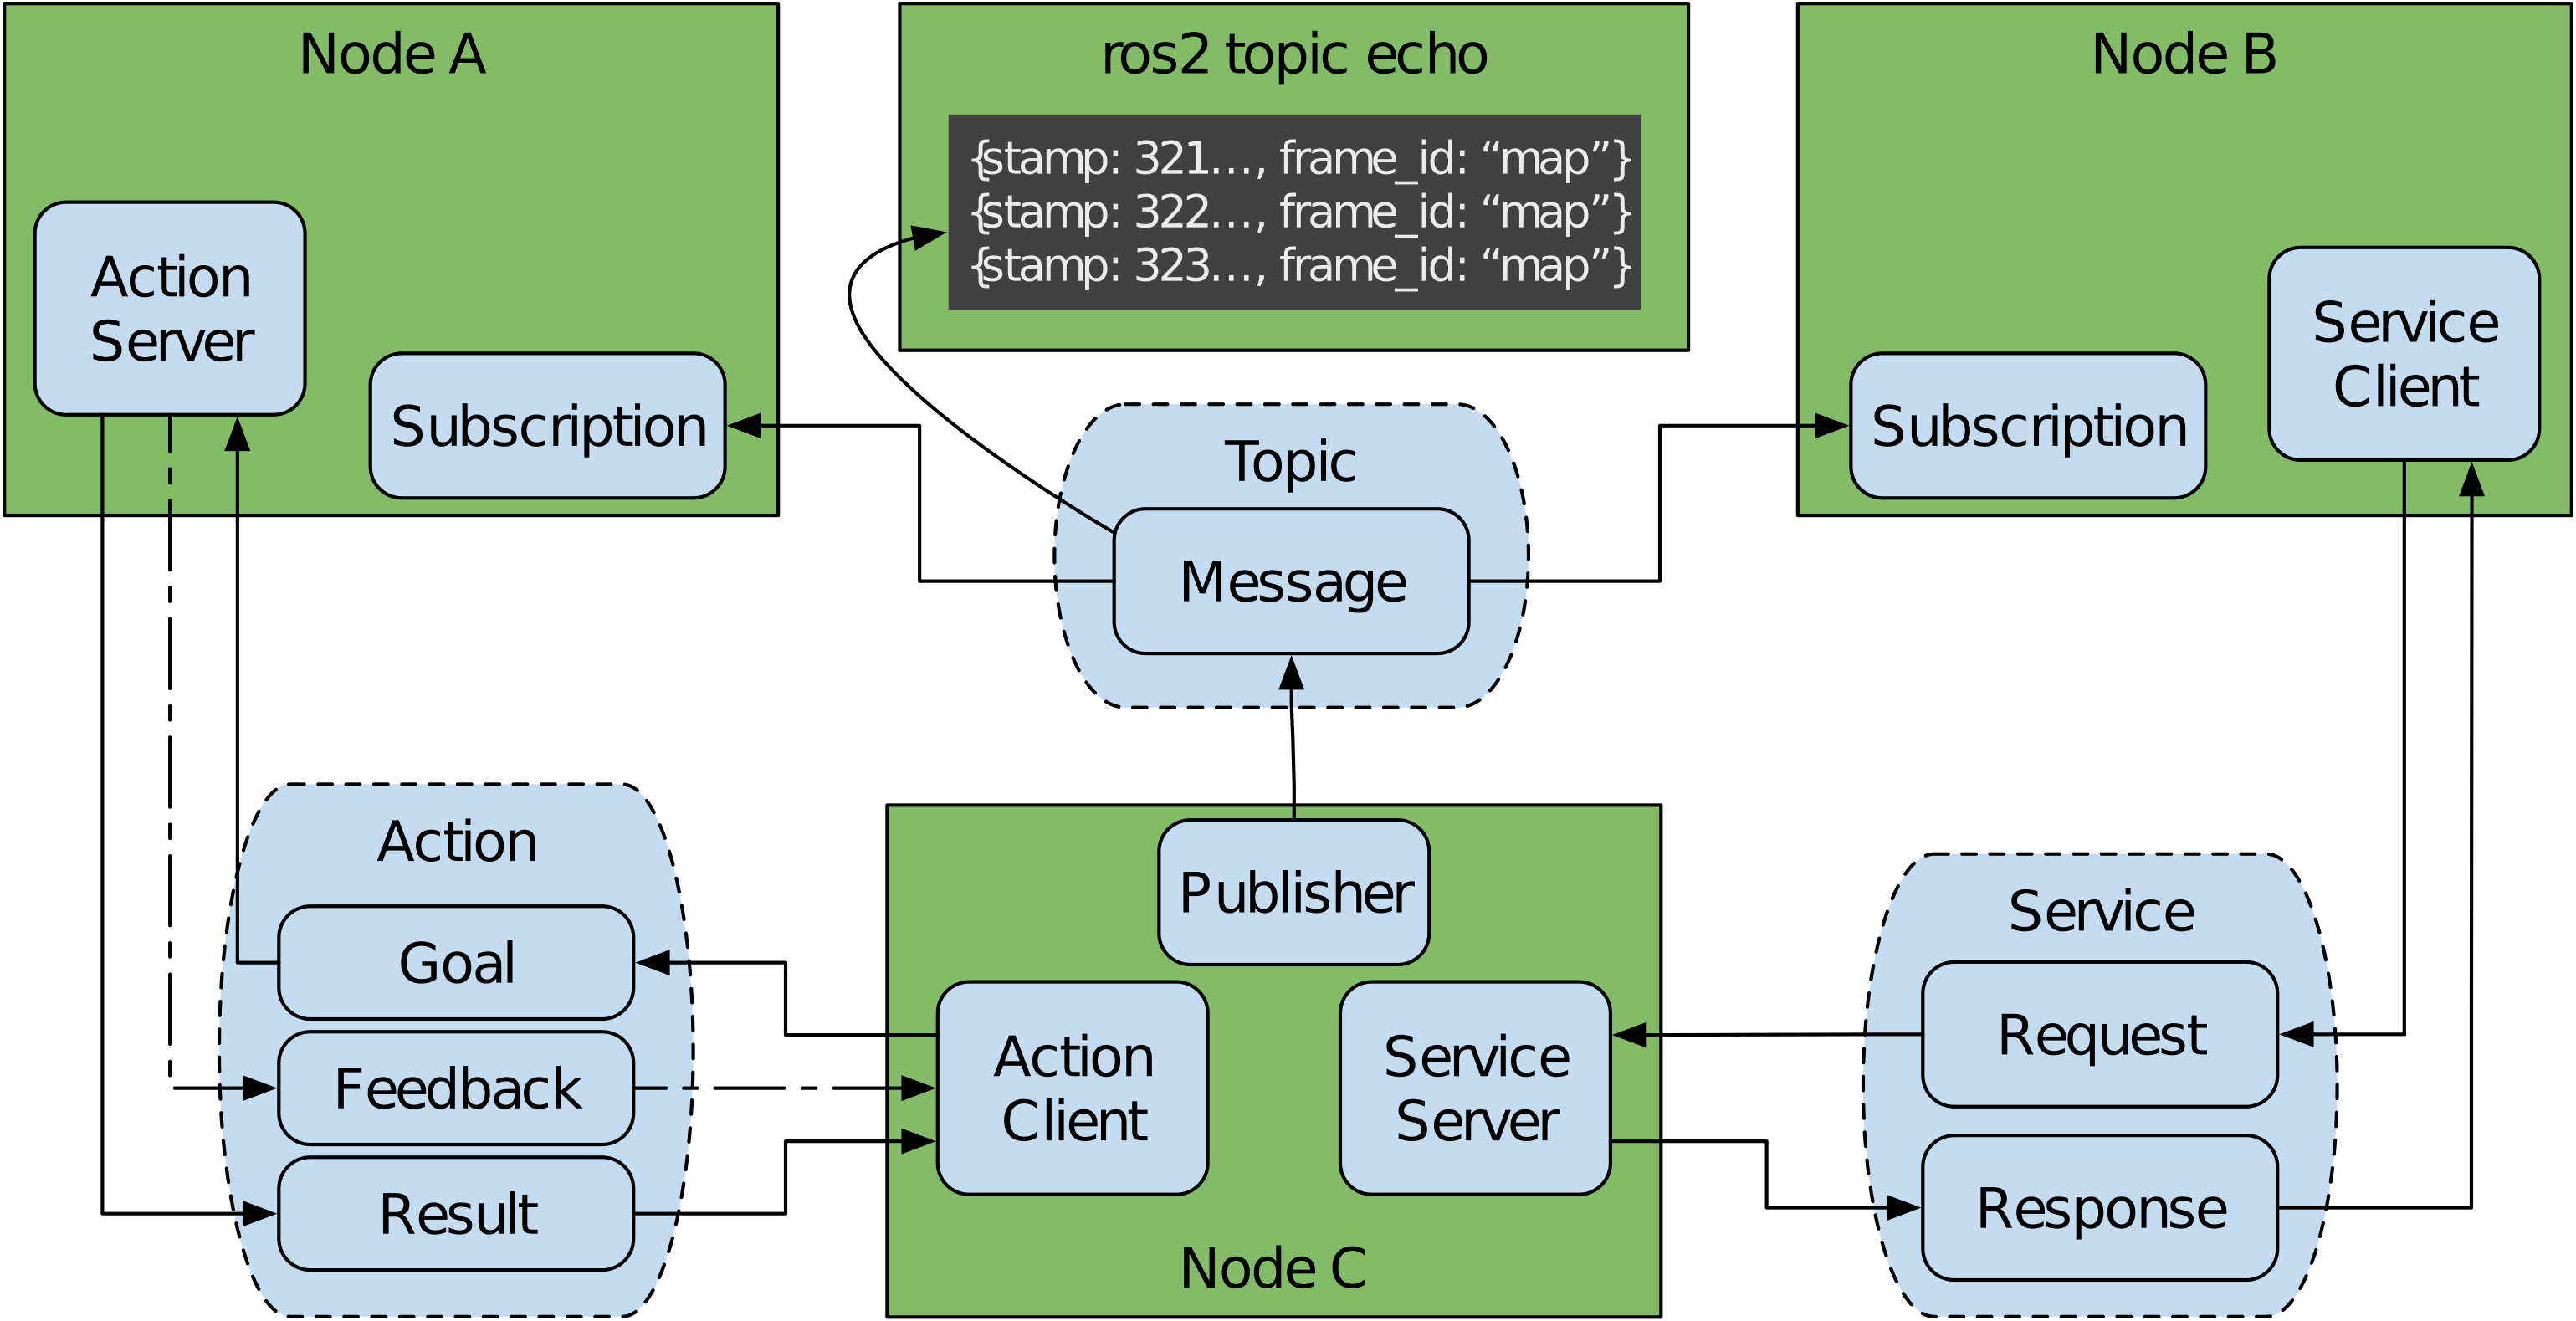
\includegraphics[width=1\linewidth]{figures/ROS2_Node_Interfaces.png}
    \caption{رابط‌های یک گره \lr{ROS2}: مبحث‌ها، سرویس‌ها، اعمال \cite{doi:10.1126/scirobotics.abm6074}}
    \label{fig:ROS2_Node_Interfaces}
\end{figure}

\subsubsection{کتابخانه‌های کلاینت}
کتابخانه‌های کلاینت،‌ واسط‌های برنامه‌نویسی هستند که به کاربران امکان پیاده‌سازی کد \lr{ROS2} را می‌دهند. با استفاده از کتابخانه‌های کلاینت،‌کاربران به مفاهیم مختلف مانند گره‌ها، مبحث‌ها، سرویس‌ها و اعمال دسترسی پیدا می‌کنند. کتابخانه‌های کلاینت، به انواع زبان‌های برنامه‌نویسی ارائه می‌شوند تا کاربران بتوانند کد ‌\lr{ROS2} خود را به زبانی که برای برنامه‌شان مناسب‌تر است،‌ بنویسند. به عنوان مثال، ممکن است کاربری بخواهد ابزار‌های تصویر‌سازی خود را با زبان پایتون\LTRfootnote{\lr{Python Programming Language}} نویسد چرا که سریع‌ترین تکرار نمونه‌سازی‌ها را داشته باشد؛ در حالی که برای بخش‌هایی از سیستم خود که به راندمان بیشتری نیاز دارد،‌ از زبان برنامه‌نویسی \lr{C++} استفاده کند  \cite{ROS2:Humble_Documentation}.

گره‌های نوشته شده با کتابخانه‌های کلاینت مختلف،‌ قادر به اشتراک‌گذاری پیام‌ها با یکدیگر هستند، زیرا تمام کتاب‌خانه‌های کلاینت \lr{ROS2}، مولدهای کدنویسی‌ای پیاده‌سازی کرده‌اند که به کاربران امکان تعامل با فایل‌های رابط \lr{ROS2}، به زبان مربوطه را می‌دهد (در فصل چهارم نیز اشاره‌ای به این موضوع می‌شود زیرا نیاز به استفاده از یک مولد است که بتوان یک سری از رابط‌های \lr{Autoware} را برای بسته‌ \lr{ROS2-For-Unity}، ترجمه کرد) \cite{ROS2:Humble_Documentation}.

\begin{figure}[h!]
    \centering
    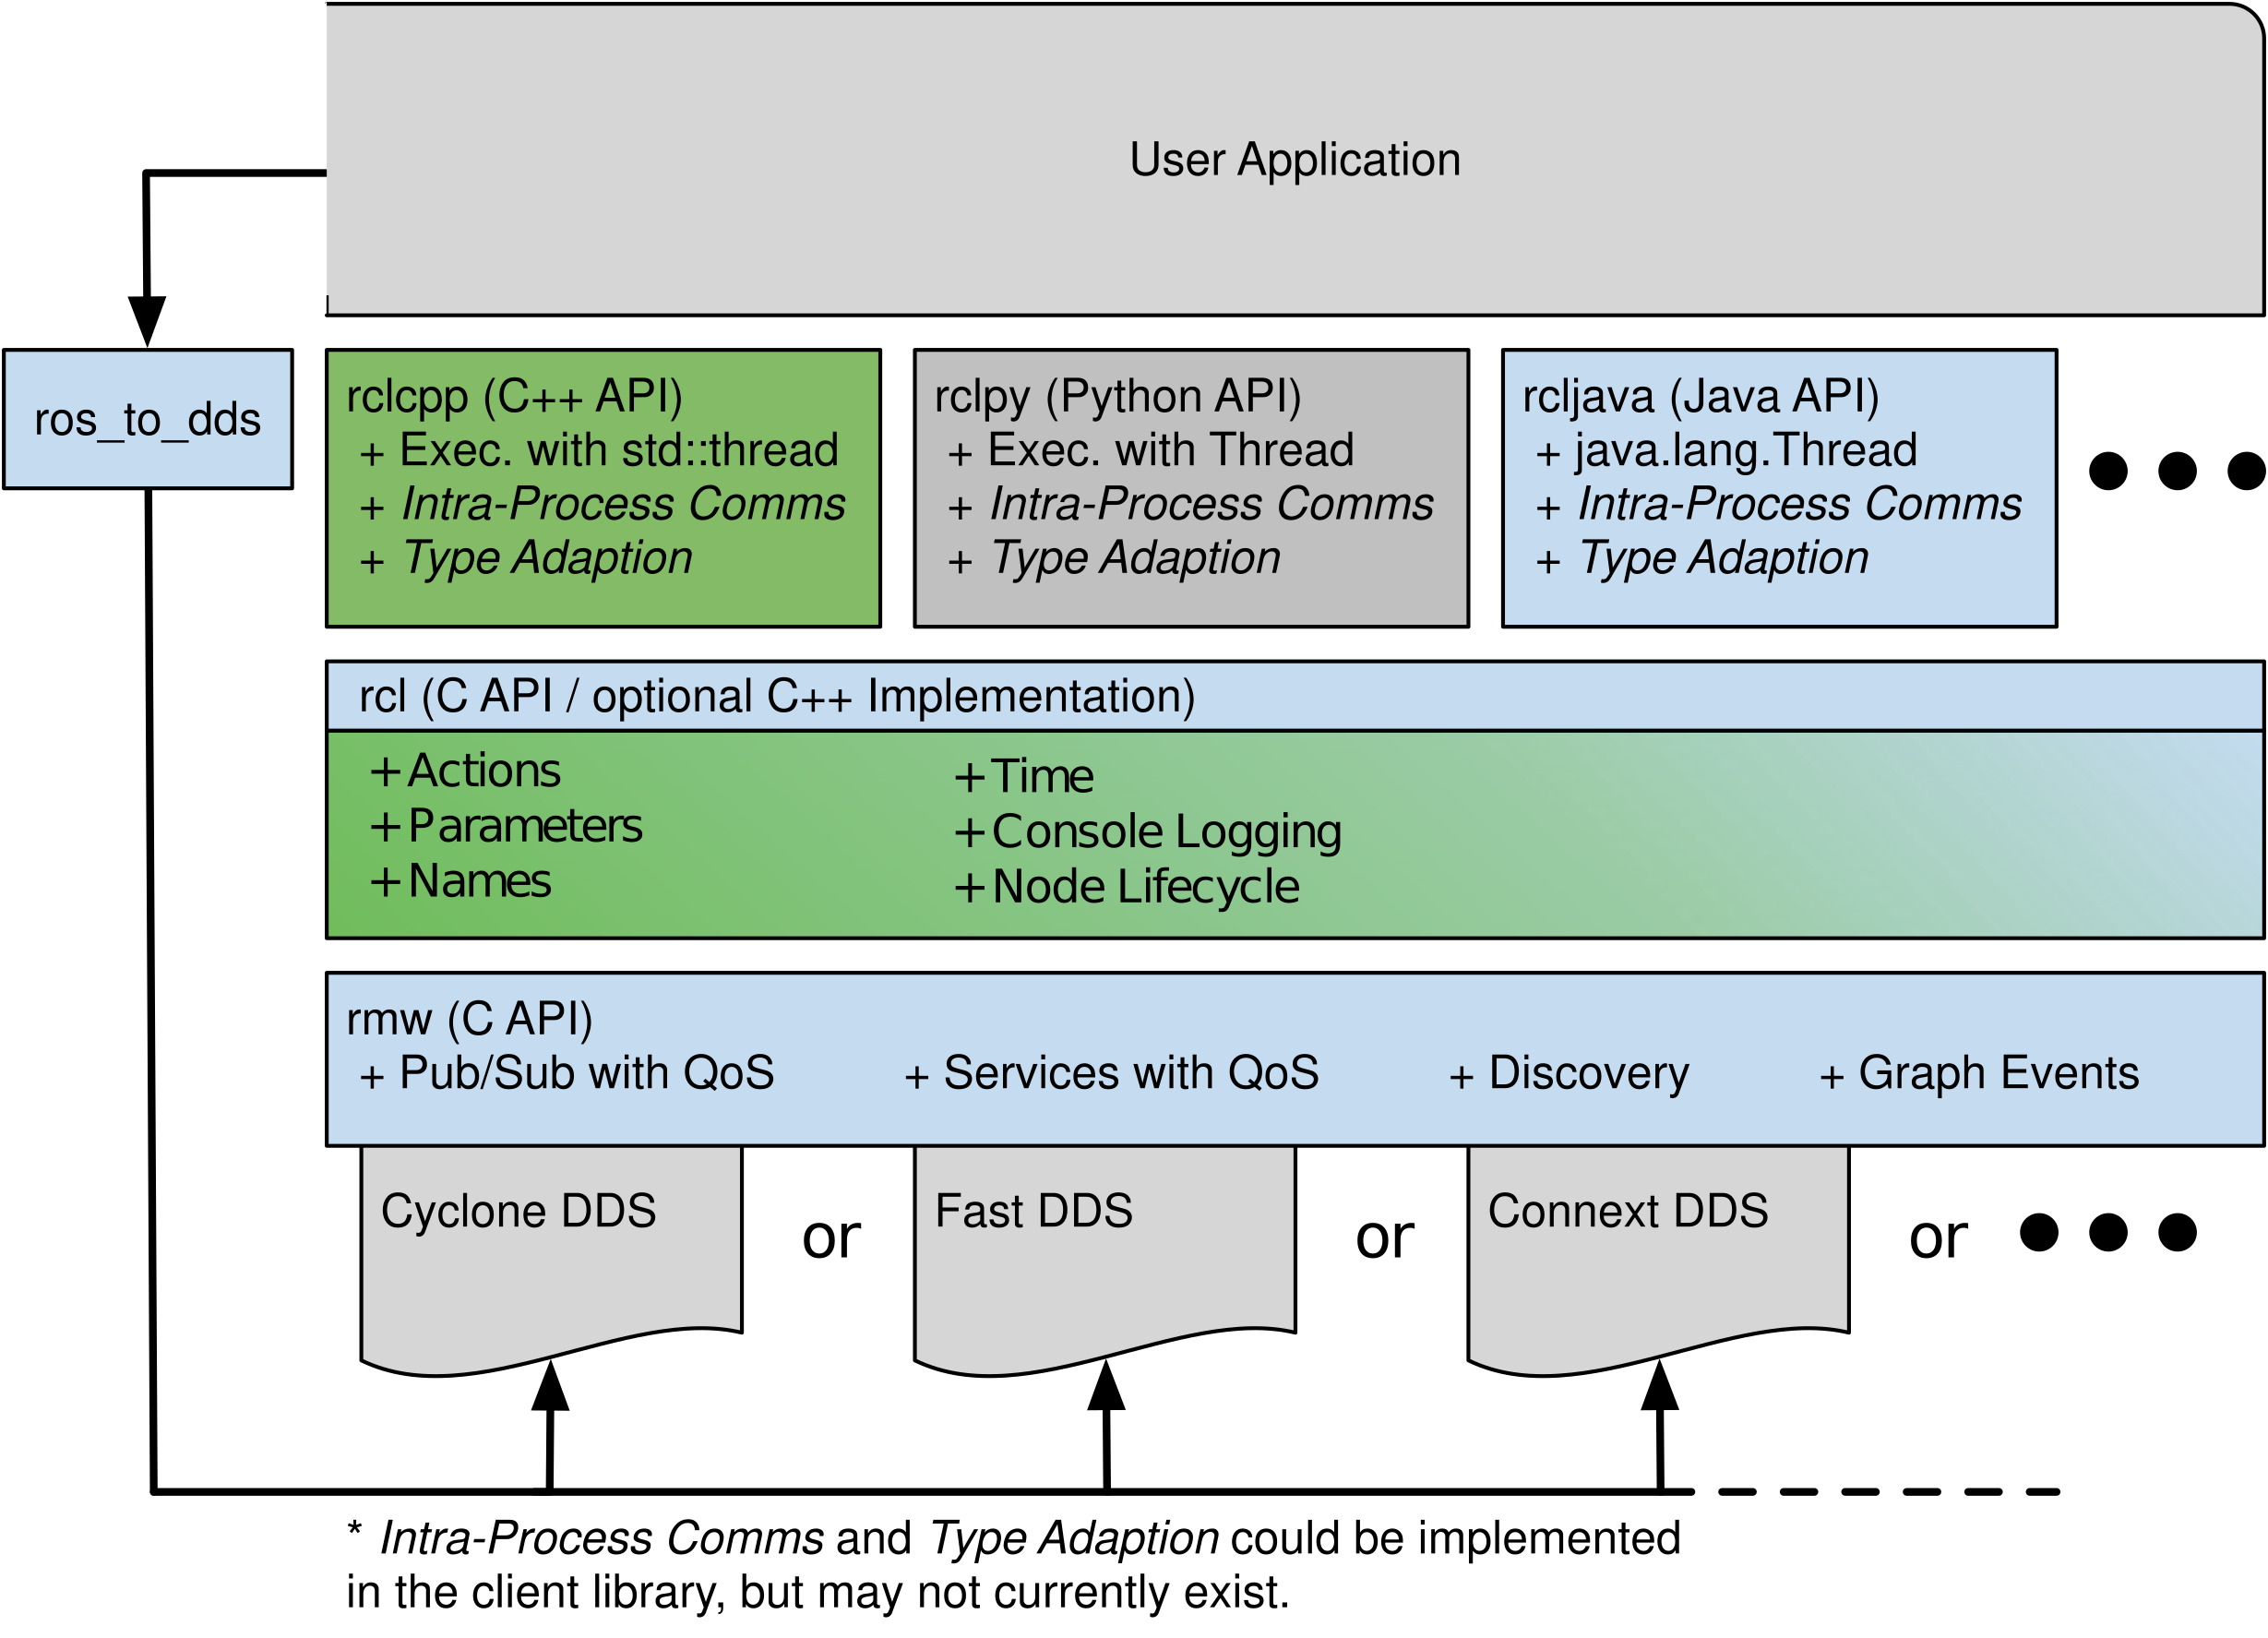
\includegraphics[width=1\linewidth]{figures/ROS2_Client_Library_API_Stack.png}
    \caption{کتابخانه‌های کلاینت \lr{ROS2} \cite{doi:10.1126/scirobotics.abm6074}}
    \label{fig:ROS2_Client_Library_API_Stack}
\end{figure}

علاوه بر ابزارهای ارتباطی مختص به زبان، کتابخانه‌های کلاینت به کاربران توانایی دسترسی به عملکرد اصلی‌ای که \lr{ROS} را به \lr{"ROS"} تبدیل می‌کند را ارائه می‌دهد. به عنوان مثال، در ادامه لیستی از عملکرد‌هایی آمده است که معمولا از طریق یک  کتابخانه کلاینت می‌توان به آنها دسترسی داشت \cite{ROS2:Humble_Documentation}:
\begin{itemize}
    \item نام‌ها و فضای نام‌ها\LTRfootnote{\lr{Namespaces}}
    \item زمان (واقعی یا شبیه‌سازی)
    \item پارامترها
    \item ثبت وقایع کنسول
    \item مدل موازی‌سازی نخ‌ها\LTRfootnote{\lr{Threading Model}}
    \item ارتباط داخلی فرایند‌ها
\end{itemize}

در \cref{fig:ROS2_Client_Library_API_Stack} نیز می‌توان کلیات نحوه کارکرد کتابخانه‌های کلاینت را مشاهده کرد.

\section{\lr{Autoware}}
نرم‌افزار \lr{Autoware} از شرکت \lr{AWF}\LTRfootnote{\lr{Autoware Foundation}}،‌ یک پشته نرم‌افزاری متن‌باز برای خودرو‌های خودران است که بر پایه \lr{ROS} ساخته شده است. این مجموعه شامل تمام عملکردهای لازم برای رانندگی خودروی خودران اعم از موقعیت‌یابی، تشخیص اجسام، برنامه‌زیری مسیر و کنترل می‌شود. هدف این مجموعه نرم‌افزار،‌ فراهم کردن بستری است که امکان مشارکت افراد و سازمان‌های مختلف در نوآوری‌های متن‌باز مربوط به فناوری‌های رانندگی خودران را می‌دهد. 

این نرم‌افزار، هم برای توسعه‌دهندگان فناوری‌های رانندگی خودران و هم برای اپراتورهای سرویس‌های این فناوری، ارزشمند است. توسعه‌دهندگان می‌توانند مولفه‌های\LTRfootnote{\lr{Component}} جدیدی را براساس \lr{Autoware}، برای خودرو‌های خودران خود پیاده‌سازی کنند. از سوی دیگر، اپراتورهای سرویس‌های خودروی خودران نیز می‌توانند از مولفه‌های مختلف \lr{Autoware}، برای فناوری خود استفاده کنند. وجود این امکانات، به علت استفاده از معماری خودمختاری در ابعاد میکرو\LTRfootnote{\lr{Microautonomy}} است، یعنی هر مولفه کوچک از این نرم‌افزار، مستقل از دیگر مولفه‌ها می‌تواند اجرا شود و اعمال تغییر در هر کدام تاثیری بر دیگر مولفه‌ها نمی‌گذارد  \cite{Autoware:Documentation}. 

\subsection{معماری خودمختار در ابعاد میکرو}
نرم‌افزار \lr{Autoware}، از معماری خط‌ لوله\LTRfootnote{\lr{Pipeline Architecture}: \url{https://www.cs.sjsu.edu/~pearce/modules/patterns/distArch/pipeline.htm}}، برای توسعه سیستم‌های خودروی خودران استفاده می‌کند. معماری خط لوله مورد استفاده در \lr{Autoware}، مولفه‌هایی دارد که مشابه معماری سه لایه‌ای\LTRfootnote{\lr{Three-Layer-Architecture}}\cite{gat1998three} عمل می‌کنند و بصورت موازی اجرا می‌شوند. دو مدول اساسی در معماری \lr{Autoware} وجود دارند:
\begin{enumerate}
    \item مدول \lr{Core}
    \item مدول \lr{Universe}
\end{enumerate}
مولفه‌های این مدول‌ها جوری طراحی شده‌اند که انعطاف پذیر و قابل استفاده مجدد باشند \cite{Autoware:Documentation}.

\begin{figure}[h!]
    \centering
    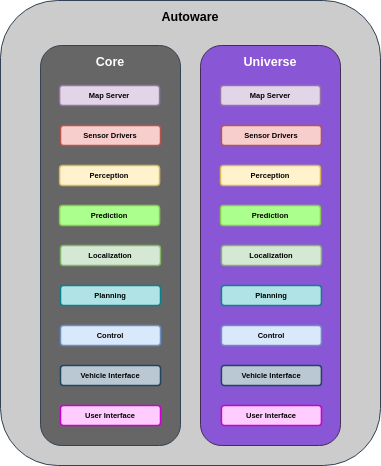
\includegraphics[width=0.5\linewidth]{figures/microautonomy_core_universe_modules.png}
    \caption{دو مدول اصلی \lr{Autoware} \cite{Autoware:Documentation}}
    \label{fig:Microautonomy_Core_Universe_Modules}
\end{figure}

\subsection{مدول \lr{Core}}
مدول \lr{Core} یا هسته، شامل برنامه‌های اجرایی‌ اساسی و مولفه‌هایی است که امکان حس کردن، محاسبه و اجرای مورد نیاز برای خودروهای خودران را فراهم می‌سازد. شرکت \lr{AWF}، مدول \lr{Core} را از طریق گروه‌های کاری خود و با معماران و اعضای برجسته‌ی خود توسعه داده و به‌روزرسانی می‌کند. هر کسی می‌تواند به مدول \lr{Core} مولفه یا کدی اضافه کند؛ اما معیارهای پذیرش این مشارکت، نسبت به مدول \lr{Universe} سخت‌گیرانه‌تر و دقیق‌تر است \cite{Autoware:Documentation}.

\subsection{مدول \lr{Universe}}
مدول‌های \lr{Universe} یا دنیا، افزونه‌هایی برای مدول \lr{Core} هستند که توسط توسعه‌دهندگان فناوری ارائه می‌شوند، تا عملکرد و توانایی حس کردن، محاسبه و اجرا را بهبود دهند. شرکت \lr{AWF}، مدول پایه \lr{Universe} را برای گسترش ارائه می‌دهد. یک ویژگی کلیدی از معماری خودمختار در ابعاد میکرو، این است که مدول‌های \lr{Universe} می‌توانند توسط مشارکت هر سازمان و فردی ساخته شوند. به عبارت دیگر، شما می‌توانید حتی مدول‌های خودتان را ایجاد کرده و برای جامعه و اکوسیستم \lr{Autoware}، در دسترس قرار دهید. شرکت \lr{AWF}، مسئول کنترل کیفیت مدول‌های \lr{Universe} در طول فرآیند توسعه آنها هستند. در نتیجه، مدول‌های \lr{Universe} دارای انواع مختلفی هستند - برخی توسط \lr{AWF} تأیید و اعتبارسنجی شده‌اند و برخی دیگر نه. انتخاب و ادغام مدول‌های \lr{Universe} برای ایجاد برنامه‌های نهایی به عهده کاربران \lr{Autoware} است. کاربران می‌توانند مولفه‌هایی از مدول \lr{Core} را با مولفه‌های \lr{Universe} که عموما بروزتر و نوین‌تر است، تعویض کنند \cite{Autoware:Documentation}.\\
\\
در ادامه، نگاهی اجمالی به مولفه‌های اصلی تشکیل‌دهنده این مدول‌ها می‌اندازیم.

\subsection{مولفه \lr{Sensing}}
مولفه \lr{Sensing} یا احساس، مجموعه‌ای از مدول‌ها است که پیش‌ پردازش‌هایی اولیه را بر روی داده‌ی ورودی از سمت حسگر‌ها، اعمال می‌کنند. ورودی‌های این مولفه در \cref{fig:Sensing_Input_Types} آمده است \cite{Autoware:Documentation}.

\begin{figure}[h!]
    \centering
    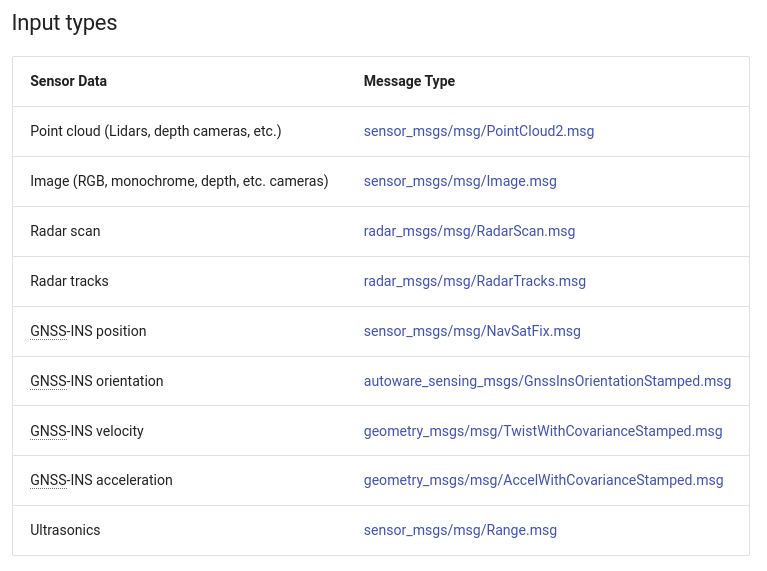
\includegraphics[width=0.64\linewidth]{figures/Sensing_Input_Types.png}
    \caption{انواع ورودی‌های قابل پذیرش توسط مولفه \lr{Sensing} \cite{Autoware:Documentation}}
    \label{fig:Sensing_Input_Types}
\end{figure}

\begin{figure}[h!]
    \centering
    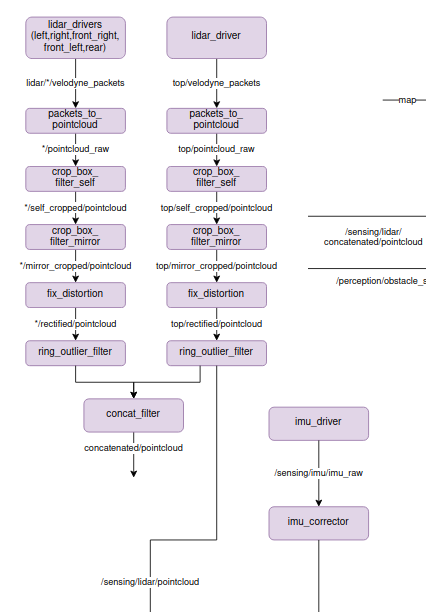
\includegraphics[width=0.75\linewidth]{figures/Sensing_Node_Graph.png}
    \caption{گراف گره‌ی مولفه ‌\lr{Sensing} \cite{Autoware:Documentation}}
    \label{fig:Sensing_Node_Graph}
\end{figure}
همانطور که در \cref{fig:Sensing_Node_Graph} مشاهده می‌شود، مبحث‌های \lr{ROS} که هر کدام از فیلتر‌های اعمال شده بر ابر‌ نقاط ورودی، به آن داده‌ منتشر ‌می‌کنند، نوشته ‌شده است\LTRfootnote{\url{https://autowarefoundation.github.io/autoware-documentation/main/design/autoware-architecture/sensing/}}.

\subsection{مولفه \lr{Map}}
نرم‌افزار \lr{Autoware}، برای انجام وظایف مختلفی نظیر موقعیت‌یابی\LTRfootnote{\lr{Localization}}، برنامه‌ریزی مسیر\LTRfootnote{\lr{Route Planning}}، تشخیص چراغ‌های راهنمایی و رانندگی، و پیش‌بینی مسیر حرکت عابر‌پیاده‌ها و دیگر وسایل نقلیه، از نقشه‌های ابر نقاط\LTRfootnote{\lr{Pointcloud Map}} با وضوح بالا و نقشه‌های برداری\LTRfootnote{\lr{Vector Map}} از محیط رانندگی، استفاده می‌کند.

مولفه \lr{Map}، بایستی دو مدل اطلاعات را برای دیگر پشته‌ها فراهم کند:
\begin{enumerate}
    \item اطلاعات معنایی\LTRfootnote{\lr{Semantic Information}} مربوط به جاده‌ها در نقشه بُرداری
    \item اطلاعات ژئومتریک\LTRfootnote{\lr{Geometric Information}} مربوط به محیط در نقشه ابر نقاط
\end{enumerate}

\begin{figure}[h!]
    \centering
    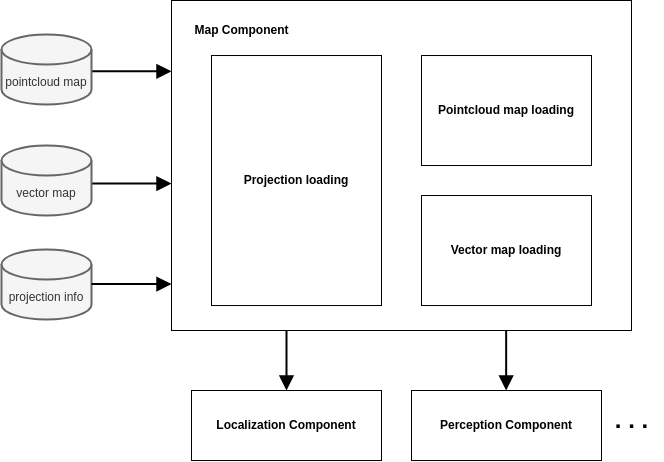
\includegraphics[width=0.75\linewidth]{figures/Autoware_Map_Architecture.png}
    \caption{معماری مولفه \lr{Map} \cite{Autoware:Documentation}}
    \label{fig:Autoware_Map_Architecture}
\end{figure}

یک نقشه بُرداری، شامل اطلاعات دقیق در مورد شبکه جاده، هندسه مسیر‌های عبوری و چراغ‌های راهنمایی و رانندگی می‌شود. این اطلاعات برای برنامه‌ریزی مسیر، تشخیص چراغ‌های راهنمایی و پیش‌بینی مسیر حرکت دیگر وسایل نقلیه و عابر‌پیاده‌ها ضروری هستند.

یک نقشه ابر نقاط سه بعدی، در درجه اول برای موقعیت‌یابی لایدار-محور و بخشی از مولفه \lr{Perception} در \lr{Autoware}، استفاده می‌شود. به منظور تعیین مکان و جهت فعلی وسیله نقلیه، اسکن زنده‌ای که از یک یا چند واحد لایدار ثبت شده است، با یک نقشه ابر نقاط سه‌بعدی پیش‌تولید شده همخوانی داده می‌شود. بنابراین، یک نقشه دقیق ابر نقاط برای نتایج خوب موقعیت‌یابی بسیار حیاتی است. با این حال، اگر وسیله نقلیه دارای یک روش موقعیت‌یابی جایگزین با دقت کافی باشد، به عنوان مثال با استفاده از موقعیت‌یابی بر اساس دوربین، احتمالاً نیازی به استفاده از نقشه ابر نقاط برای وجود نخواهد داشت \cite{Autoware:Documentation}. در \cref{fig:Autoware_Map_Architecture}، معماری‌ سطح‌ بالایی از مولفه \lr{Map} را مشاهده می‌کنیم  \LTRfootnote{\url{https://autowarefoundation.github.io/autoware-documentation/main/design/autoware-architecture/map/}}.

\begin{figure}[h!]
    \centering
    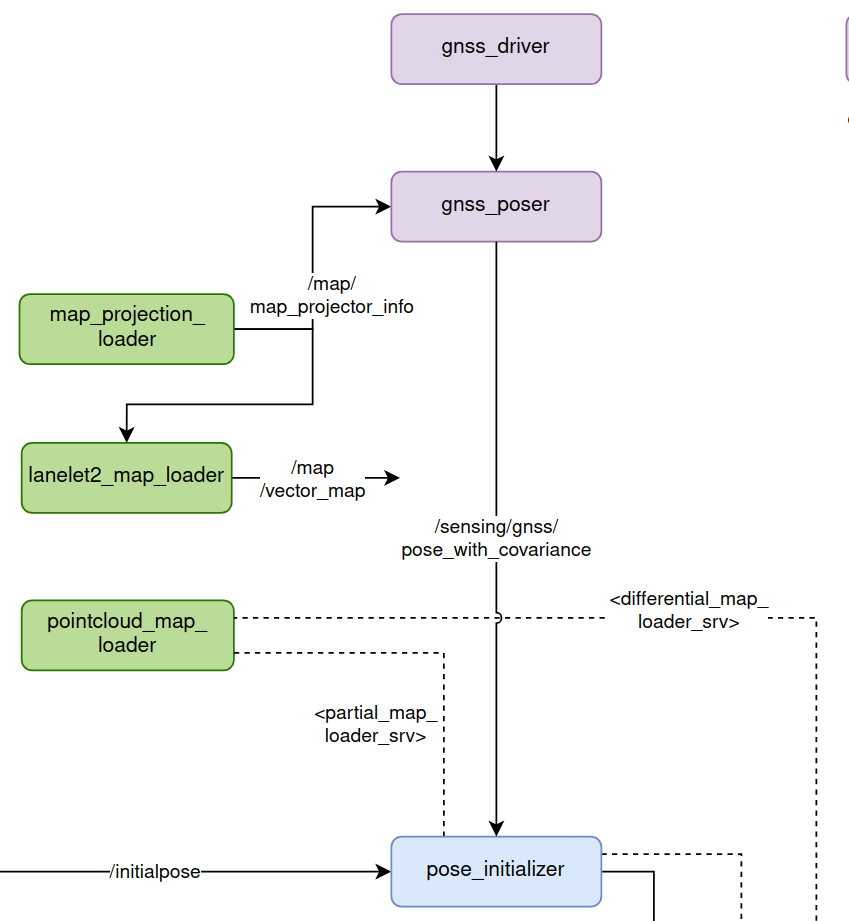
\includegraphics[width=0.75\linewidth]{figures/Autoware_Map_Node_Graph.png}
    \caption{گراف گره‌ی مولفه \lr{Map} (مستطیل‌های سبز) \cite{Autoware:Documentation}}
    \label{fig:Autoware_Map_Node_Graph}
\end{figure}

\subsection{مولفه \lr{Localization}}
مولفه \lr{Localitzation} یا موقعیت‌یابی، سعی در تخمین موقعیت، سرعت و شتاب خودروی خودران دارد. همچنین سعی شده است تا سیستمی طراحی شود که عملیات موقعیت‌یابی را با حسگر‌های مختلف انجام دهد و در صورتی که تخمین با خطای زیادی مواجه باشد، پیام هشداری را به سیستم نظارتی خودروی خودران ارسال کند.
این مولفه، با پیکربندی حسگر‌های مختلف زیر کار می‌کند:
\begin{enumerate}
    \item لایدار سه‌بعدی + نقشه ابر نقاط
    \item لایدار سه‌بعدی یا دوربین + نقشه بُرداری
    \item  دوربین (ادومتری بصری،‌ محلی‌سازی و نقشه‌برداری همزمان\LTRfootnote{\lr{SLAM: Simultaneous Localization And Mapping}} بصری)
    \item حسگر سرعت چرخ
    \item واحد اندازه‌گیری لختی \LTRfootnote{\lr{IMU: Inertial Measurement Unit}}
    \item حسگر ژئو-مغناطیسی\LTRfootnote{\lr{Geomagnetic Sensor}}
    \item نشانگرهای مغناطیسی\LTRfootnote{\lr{Magnetic Markers}}
\end{enumerate}

در \cref{fig:Autoware_Localization_Architecture}، معماری‌ پیشنهادی، که توسط توسعه‌دهندگان \lr{Autoware} برای توسعه‌دهندگان دیگر در اختیار گذاشته‌اند، مشاهده می‌شود. برای دقت بالا در موقعیت یابی، پیشنهاد شده است که واحد اندازه‌گیری لختی و حسگر لایدار حتما استفاده شوند؛ همچنین نقشه بُرداری و نقشه ابر نقاط محیط نیز به عنوان ورودی به مولفه \lr{Localization} داده شوند \cite{Autoware:Documentation}.

\begin{figure}[h!]
    \centering
    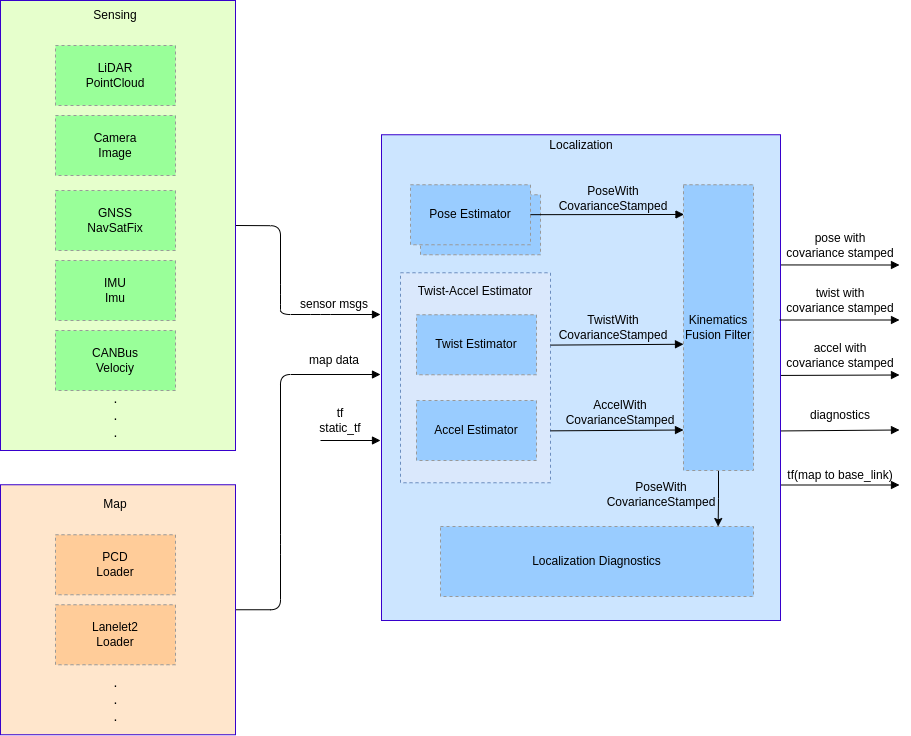
\includegraphics[width=0.75\linewidth]{figures/Autoware_Localization_Architecture.png}
    \caption{معماری پیشنهادی \lr{Autoware} برای مولفه \lr{Localization} \cite{Autoware:Documentation}}
    \label{fig:Autoware_Localization_Architecture}
\end{figure}

\begin{figure}[h!]
    \centering
    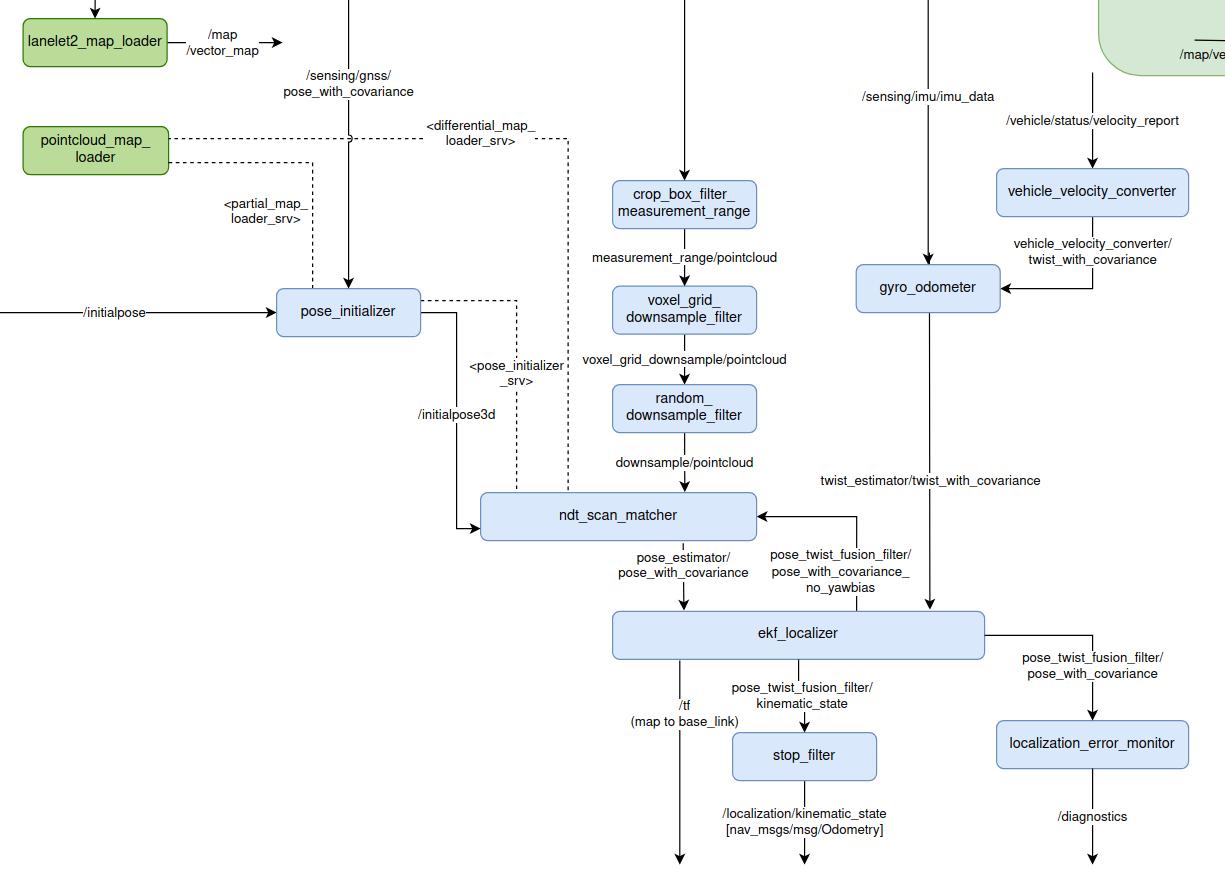
\includegraphics[width=0.85\linewidth]{figures/Autoware_Localization_Node_Graph.png}
    \caption{گراف گره‌ی مولفه \lr{Localization} \cite{Autoware:Documentation}}
    \label{fig:Autoware_Localization_Node_Graph}
\end{figure}

\subsection{مولفه \lr{Perception}}
مولفه \lr{Perception} یا ادراک، وظیفه‌ی تشخیص انواع وسایل نقیه مانند خودرو، کامیون، موتور، اتوبوس، و همچنین عابرین پیاده را بر عهده دارد. این مولفه، علاوه بر تشخیص اجسام سه‌بعدی ذکر شده، شناسه‌ی یکتایی را به آنها نسبت می‌دهد و آنها را ردیابی\LTRfootnote{\lr{Track}}  می‌کند تا موقعیت، شتاب، سرعت، مسیر حرکت و جهت قرارگیری آنها را محاسبه کند. این مولفه در مدول \lr{Universe} دارای الگوریتم‌های گوناگونی برای ادراک محیط است و ورودی‌های آن همانند مولفه \lr{Sensing} می‌باشد. این مولفه از چند گره اصلی تشکیل شده است:
\begin{enumerate}
    \item گره‌ پیش‌پردازش
    \item گره تشخیص  و ردیابی اجسام سه‌بعدی
    \item گره تشخیص علایم راهنمایی و رانندگی
    \item گره پیش‌بینی مسیر حرکت اجسام
    \item گره پس‌پردازش
\end{enumerate}

بایستی توجه داشت که ورودی‌های ابر نقاط لایدار، برای این مولفه ضروری است و نداشتن آن، دقت تشخیص را به مراتب کاهش می‌دهد. در معماری رابط‌های مولفه \lr{Perception}، مشاهده می‌شود. همانطور که ذکر شد، پیشنهاد می‌شود که حتما از داده‌های ابر نقاط برای تشخیص اجسام استفاده کرد.

\begin{figure}[h!]
    \centering
    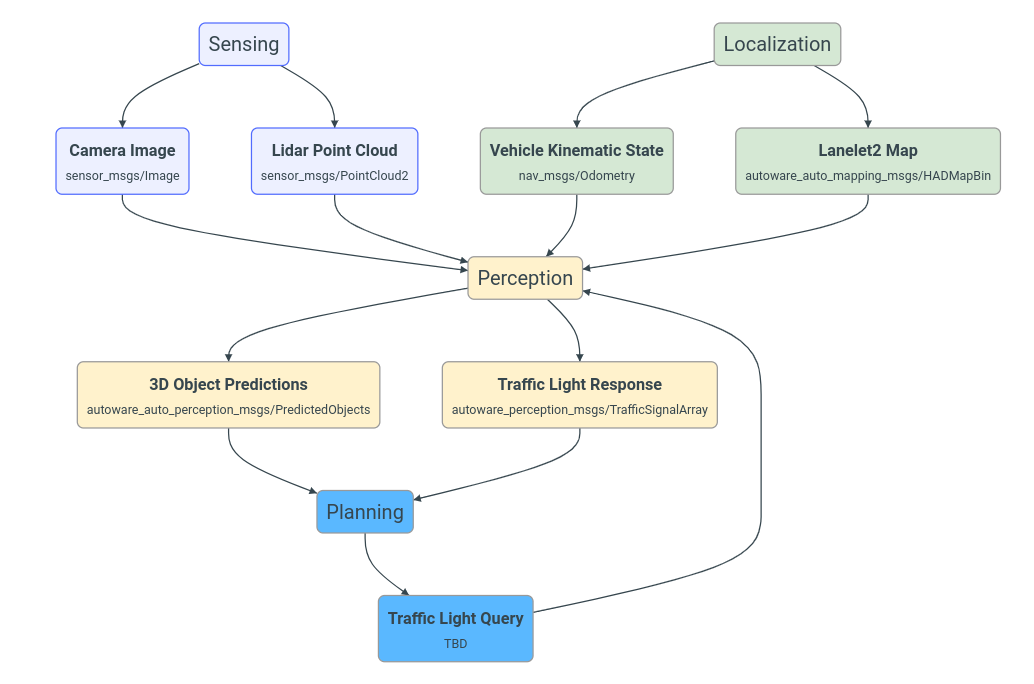
\includegraphics[width=0.85\linewidth]{Autoware_Perception_Interface_Architecture.png}
    \caption{معماری رابط‌های مولفه \lr{Perception} \cite{Autoware:Documentation}}
    \label{fig:Autoware_Perception_Interface_Architecture}
\end{figure}

از آنجایی که در این پژوهش، از این مولفه استفاده شده است، لازم است تا برخی از گره‌های مهم آن توضیح داده شوند.

\subsubsection{گره پیش‌پردازش}
این گره وظیفه اعمال فیلترهایی اولیه به ابر نقاط ورودی را بر عهده دارد. 

\begin{figure}[h!]
    \centering
    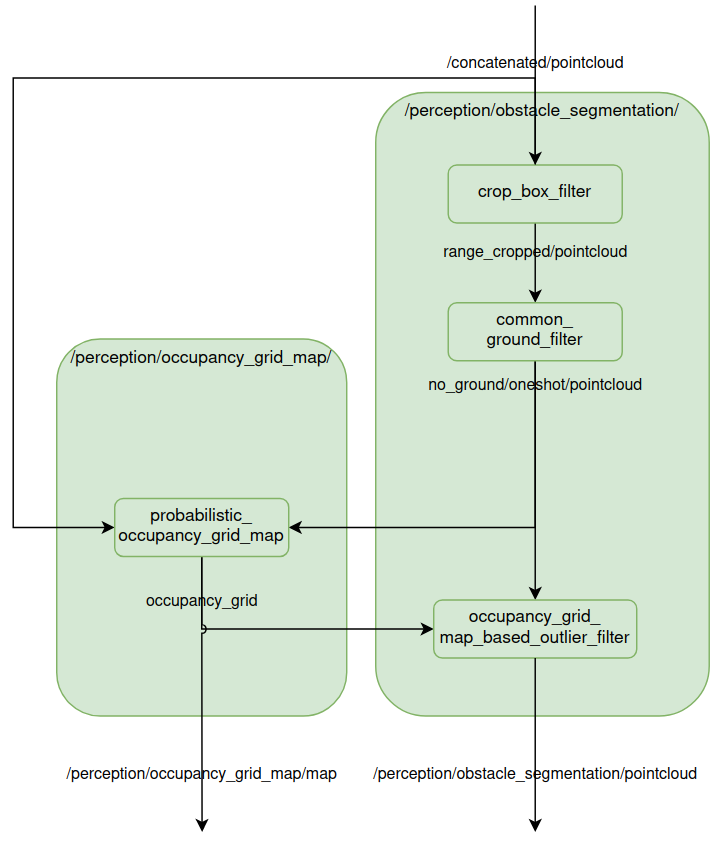
\includegraphics[width=0.45\linewidth]{figures/Autoware_Perception_Preprocessing_Node_Graph.png}
    \caption{ گراف گره‌ی پیش‌پردازش مولفه \lr{Perception} \cite{Autoware:Documentation}}
\label{fig:Autoware_Perception_Preprocessing_Node_Graph}
\end{figure}

طبق \cref{fig:Autoware_Perception_Preprocessing_Node_Graph} مشاهده می‌کنیم که گره پیش‌پردازش، خود از گره‌هایی کوچک‌تر ساخته شده‌اند که عبارتند از:
\begin{enumerate}
    \item فیلتر \lr{crop\_box}: این گره با استفاده از کتابخانه \lr{PCL}\LTRfootnote{\lr{Point Cloud Library} : \url{https://pcl.readthedocs.io/projects/tutorials/en/master/\#}} تمام نقاطی که در یک منطقه مکعبی مشخص شده باشد را از ابر نقاط حذف می‌کند. از این گره برای فیلتر کردن نقاطی که مربوط به خود خودروی  خودران است، استفاده می‌شود.
    \item فیلتر \lr{common\_ground}:‌ این گره برای حذف نقاط زمین از ابر نقاط استفاده می‌کند\LTRfootnote{\url{https://autowarefoundation.github.io/autoware.universe/main/perception/ground_segmentation/}}. 
    \item نقشه شبکه اشغال احتمالاتی\LTRfootnote{\lr{Probabilistic Occupancy Grid Map}}: از این گره برای ساختن نقشه‌ای از احتمال وجود موانع در اطراف ماشین خودران، استفاده می‌شود\LTRfootnote{\url{https://autowarefoundation.github.io/autoware.universe/main/perception/probabilistic_occupancy_grid_map/}}.
\end{enumerate}

\subsubsection{گره تشخیص و ردیابی اجسام سه‌بعدی}
در این گره که همانند گره پیش‌پردازش از چندین گره کوچکتر ساخته شده است، ابر نقاط فیلتر شده به عنوان ورودی به مدل‌ تشخیص‌دهنده اجسام سه‌بعدی داده می‌شود و سپس بر روی کادر محصور‌کننده خروجی این مدل، الگوریتم‌های ردیابی زده می‌شود. در \cref{fig:Autoware_Perception_Detection_Node_Graph} معماری گره تشخیص مشاهده می‌شود. همانطور که از شکل معلوم است، گره \lr{Perception} از گره‌های کوچکتری تشکیل شده است که عبارتند از:
\begin{enumerate}
    \item گره تشخیص دهنده سه‌بعدی \lr{(lidar\_centerpoint)}: این گره، یک مدل هوش مصنوعی تشخیص سه‌بعدی ابر نقاط-محور مبتنی بر واکسل، به نام \lr{Centerpoint} است \cite{yin2021center}. ابر نقاط فیلتر شده به عنوان ورودی به این تشخیص دهنده داده‌ می‌شود و کادر‌های محصور کننده اجسام تشخیص داده شده، به عنوان خروجی دریافت می‌شوند. این مدل هوش مصنوعی، از یک شبکه عصبی بر مبنای \lr{PointPillars} \cite{lang2019pointpillars} استفاده می‌کند. این شبکه عصبی با بهره‌وری از کتابخانه \lr{TensorRT}\LTRfootnote{\url{https://developer.nvidia.com/tensorrt}}، که برای سرعت‌های بسیار بالا (تشخیص بلادرنگ) و استفاده بهینه از کارت گرافیکی ساخته شده است، پیاده‌سازی شده است.
    \item گره اعتبار سنجی موانع براساس ابر نقاط \lr{(obstacle\_pointcloud\_based\_validator)}: این گره، خروجی مدل هوش‌ مصنوعی را بررسی می‌کند و اجسامی که از مجموعه نقاط کمی تشکیل شده باشند را به عنوان مثبت‌های کاذب تشخیص داده و حذف می‌کند.
    \begin{figure}[h!]
    \centering
    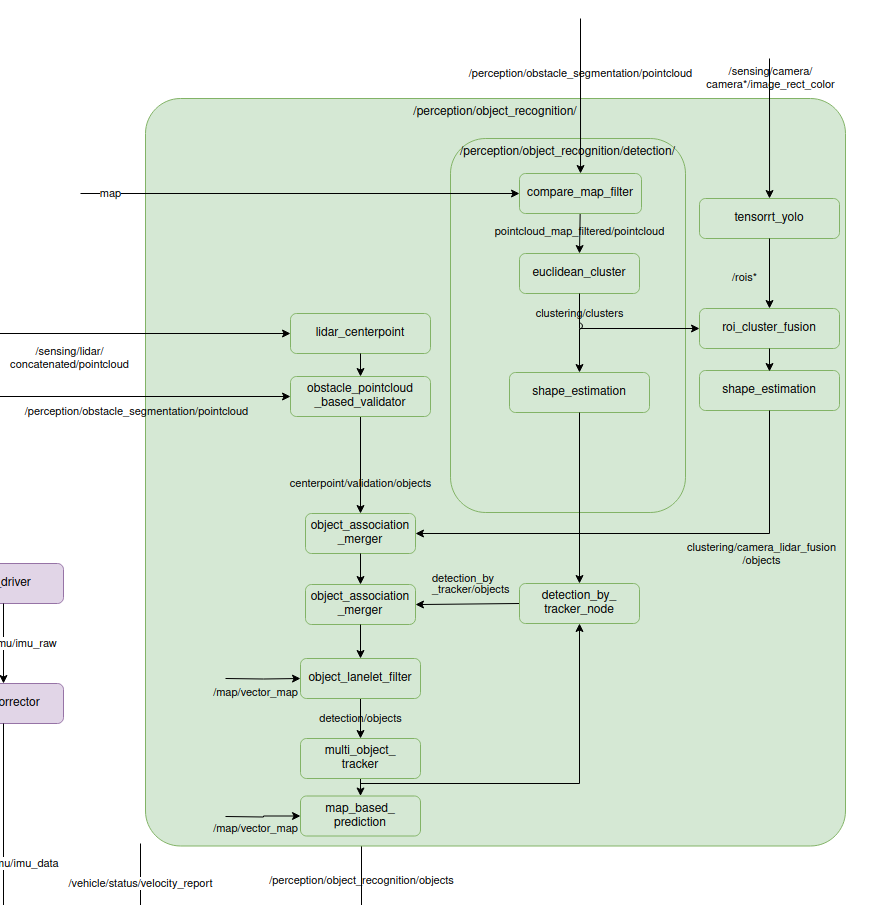
\includegraphics[width=1\linewidth]{figures/Autoware_Perception_Detection_Node_Graph.png}
    \caption{گراف گره‌‌ی تشخیص اجسام و ردیابی مولفه \lr{Perception} \cite{Autoware:Documentation}}
    \label{fig:Autoware_Perception_Detection_Node_Graph}
    \end{figure}
    \item گره فیلتر مقایسه نقشه \lr{(compare\_map\_filter)}: این گره برای تشخیص نقاط مربوط به زمین و حذف آن‌ها با استفاده از نقشه ابر نقاط است\LTRfootnote{\url{https://autowarefoundation.github.io/autoware.universe/main/perception/compare_map_segmentation/}}.
    \item گره خوشه‌بندی اقلیدسی \lr{(euclidean\_cluster)}: این گره، با استفاده از خوشه‌بندی اقلیدسی کتابخانه \lr{PCL}، اقدام به خوشه‌بندی ابر نقاط می‌کند که از آن برای تشخیص اجسام و همچنین تشخیص ابعاد اجسام استفاده می‌شود\LTRfootnote{\url{https://autowarefoundation.github.io/autoware.universe/main/perception/euclidean_cluster/}}.
    \item گره تخمین شکل \lr{(shape\_estimation)}: این گره، شکل دقیق‌تری از جسم (کادر محصورکننده \cite{Zhang-2017-26536}، استوانه، پوشش محدب\LTRfootnote{\lr{Convex Hull}}) را که خوشه‌ی ابر نقاط در ارتباط با یک برچسب، در آن جا می‌شود را محاسبه می‌کند.
    \item گره ادغام کننده اجسام \lr{(object\_association\_merger)}: این گره اجسام تشخیص داده‌ شده از دو روش تشخیص اجسام مختلف را ادغام می‌کند\LTRfootnote{\url{https://autowarefoundation.github.io/autoware.universe/main/perception/object_merger/}}.
    \item گره فیلتر لینلت \lr{(object\_lanelet\_filter)}: این گره، اجسام تشخیص داده شده را براساس نقشه بُرداری فیلتر می‌کند. این گره تنها اجسامی که داخل خطوط جاده‌ها و پیاده‌رو‌ها باشند را از فیلتر عبور می‌دهد\LTRfootnote{\url{https://autowarefoundation.github.io/autoware.universe/main/perception/detected_object_validation/object-lanelet-filter/}}.
    \item گره ردیاب هم‌زمان چند جسم \lr{(multi\_object\_tracker)}: نتایج تشخیص اجسام، توسط یک سری زمانی پردازش می‌شوند. هدف اصلی، دادن شناسه یکتا به هر یک از اجسام تشخیص داده شده و تخمین سرعت ‌آن‌ها است\LTRfootnote{\url{https://autowarefoundation.github.io/autoware.universe/main/perception/multi_object_tracker/}}.
    \item گره تشخیص براساس ردیاب \lr{(detection\_by\_tracker)}: این گره، اجسام ردیابی شده را به گره تشخیص باز می‌گرداند تا پایدار بماند و به شناسایی اجسام ادامه دهد. این گره یک جسم ناشناخته حاوی یک خوشه نقاط و یک ردیاب را به عنوان ورودی، دریافت می‌کند. جسم ناشناخته تا مرحله متناسب شدن با ابعاد ردیاب، بهینه ‌می‌شود تا بتواند به شناسایی شدن ادامه دهد. 
    گره‌ی تشخیص با استفاده از ردیاب، یک شئ ناشناخته شامل یک ابر نقطه و یک ردیاب دریافت می‌کند، سپس شکل شیء ناشناخته با استفاده از خوشه‌بندی اقلیدسی، متناسب می‌شود. متناسب‌سازی شکل با استفاده از خوشه‌بندی اقلیدسی و روش‌های دیگر مشکلی به نام کم‌تقسیم‌بندی\LTRfootnote{\lr{Under-Segmentation}} و بیش‌تقسیم‌بندی\LTRfootnote{\lr{Over-Segmentation}} دارد، که با اعمال سیاست‌هایی بهبود می‌یابد\LTRfootnote{\url{https://autowarefoundation.github.io/autoware.universe/main/perception/detection_by_tracker/}} \cite{Autoware_Universe:Documentation}.
\end{enumerate}

\subsection{مولفه \lr{Planning}}
مولفه \lr{Planning} یا برنامه‌ریزی مسیر، پیام مسیر پیشنهادی را براساس وضعیت محیط که از مولفه‌های ادراک و موقعیت‌یابی بدست می‌آورد، منتشر می‌کند و مولفه \lr{Control} از این پیام استفاده می‌کند.

\begin{figure}[h!]
    \centering
    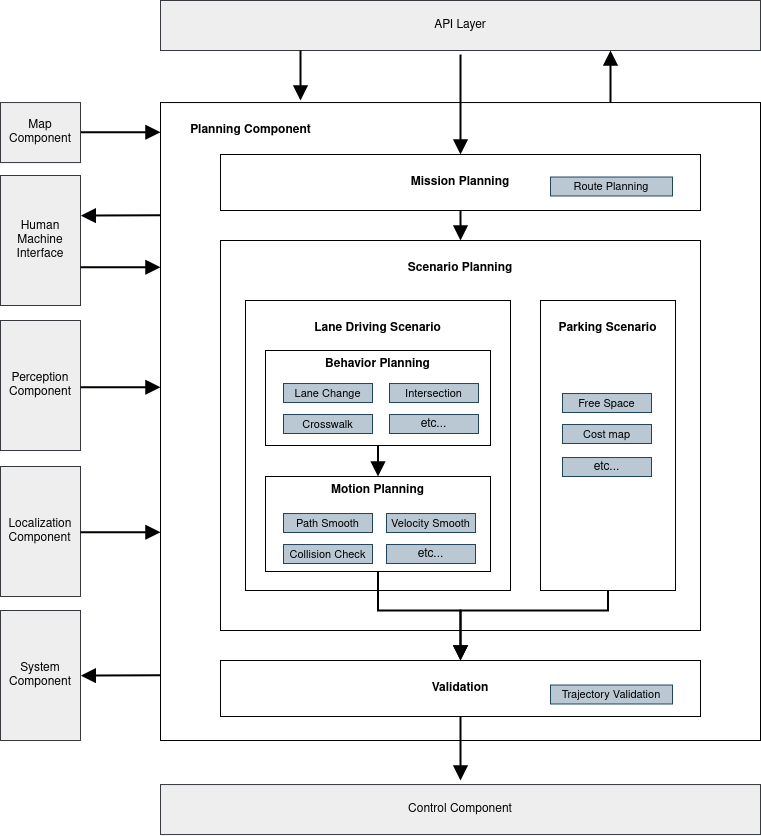
\includegraphics[width=0.75\linewidth]{figures/Autoware_Planning_Architecture.png}
    \caption{معماری سطح بالای مولفه \lr{Planning} \cite{Autoware:Documentation}}
    \label{fig:Autoware_Planning_Architecture}
\end{figure}

همانطور که طبق \cref{fig:Autoware_Planning_Architecture} مشاهده می‌شود، مولفه \lr{Planning} از چند مولفه کوچک‌تر ساخته شده است:
\begin{enumerate}
    \item مولفه برنامه‌ریزی ماموریت \lr{(Mission Planning)}:‌ مسیر را براساس هدف و اطلاعات نقشه  داده شده، محاسبه می‌کند.
    \item مولفه برنامه‌ریزی سناریو \lr{(Scenario Planning)}: مسیر را براساس سناریو حال حاضر تعیین می‌کند (به طور مثال سناریو رانندگی در خطوط جاده یا سناریو پارک کردن).
    \begin{itemize}
        \item مولفه رانندگی در خطوط \lr{(Lane Driving)}: مسیر را برای رانندگی در بین خطوط جاده را محاسبه می‌کند.
        \item مولفه برنامه‌ریزی رفتار \lr{(Behavior Planner)}: مسیر مطلوب را براساس ملاحظات ایمنی و قوانین راهنمایی رانندگی، محسابه می‌کند.
        \item مولفه برنامه‌ریزی حرکت \lr{(Motion Planner)}: مسیر مطلوب خودرو را براساس عامل‌های ایمنی، ملاحظات سرعت خودرو و دستورات مولفه برنامه‌ریزی رفتار، محسابه می‌کند.
        \item مولفه پارک کردن \lr{(Parking)}: مسیر را در سناریوهای پارک کردن در جای ناشناخته، محاسبه می‌کند.
    \end{itemize}
    \item مولفه اعتبارسنجی \lr{(Validation)}: ایمن بودن مسیر محاسبه شده را می‌سنجد.
\end{enumerate}

هر کدام از مولفه‌ها می‌توانند براساس وضعیت، به صورت پویا اضافه و حذف شوند. این معماری، برگرفته از معماری خودمختار در ابعاد میکرو نرم‌افزار \lr{Autoware} است، که این اجازه را می‌دهد که هر کدام از مولفه‌ها نسبت به شرایط، به خط‌ لوله اجرایی اضافه یا از آن حذف شوند \cite{Autoware:Documentation}. 

برای مشاهده گراف گره این مولفه، می‌توان به صفحه گراف گره کلی \lr{Autoware} مراجعه کرد\LTRfootnote{\url{https://autowarefoundation.github.io/autoware-documentation/main/design/autoware-architecture/node-diagram/}}. همچنین دو مولفه پایانی \lr{Control} و \lr{Vehicle}، به علت مربوط نبودن به پژوهش، توضیح داده نمی‌شوند. \cref{fig:Autoware_Architecture}،‌ معماری کلی نرم‌افزار \lr{Autoware} را در یک نگاه نشان می‌دهد.

\begin{figure}[h!]
    \centering
    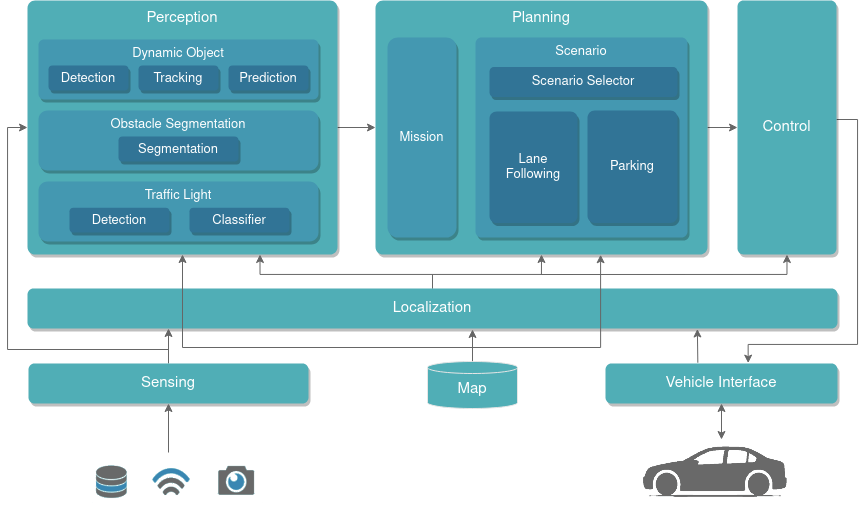
\includegraphics[width=1\linewidth]{figures/Autoware_Architecture.png}
    \caption{معماری سطح‌‌بالای نرم‌افزار \lr{Autoware} \cite{Autoware:Documentation}}
    \label{fig:Autoware_Architecture}
\end{figure}

\section{شبیه‌ساز \lr{AWSIM}}
\begin{figure}[h!]
    \centering
    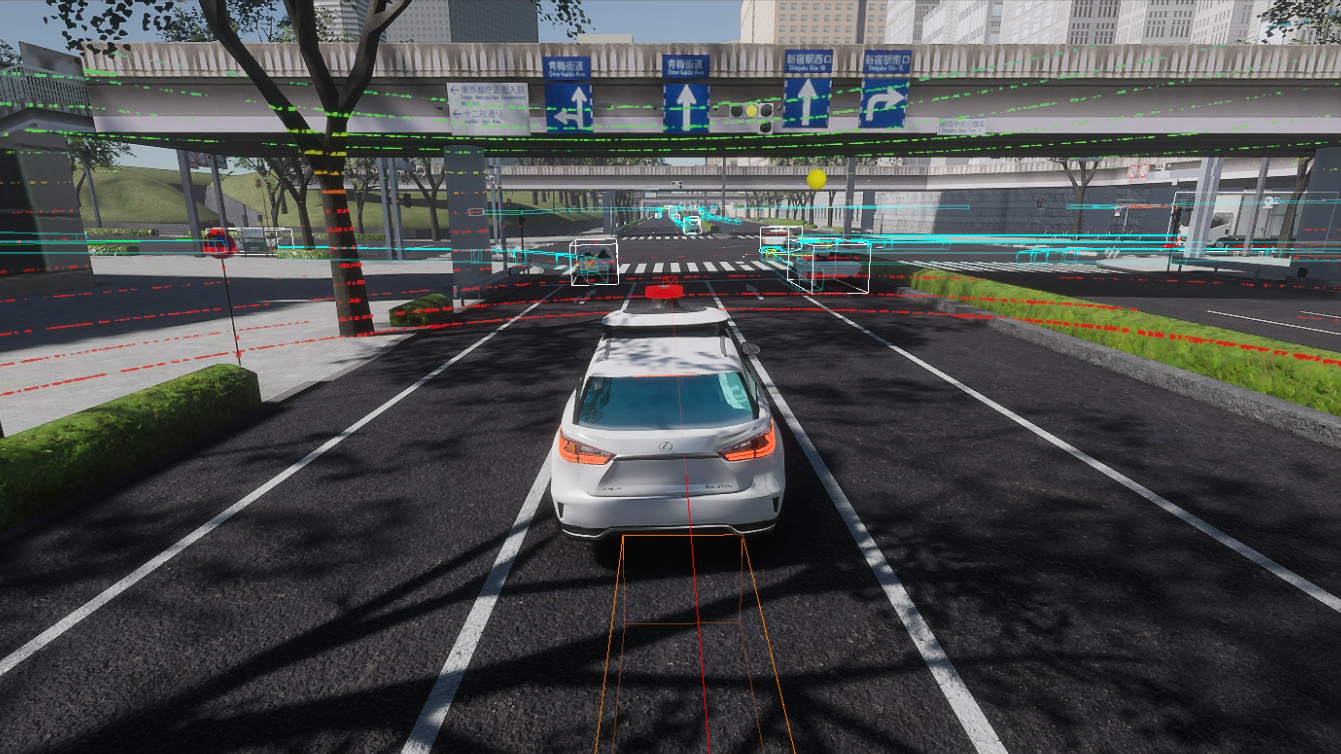
\includegraphics[width=1\linewidth]{figures/E2ESim.png}
    \caption{شبیه‌ساز \lr{AWSIM} \cite{AWSIM:Documentation}}
    \label{fig:AWSIM}
\end{figure}

\lr{AWSIM} یک شبیه‌ساز متن‌باز ساخته شده با استفاده از موتور بازی‌سازی \lr{Unity} است که برای تحقیق و توسعه در حوزه رانندگی خودکار است. این شبیه‌ساز برای نرم‌افزارهای خودروی خودران همانند \lr{Autoware}، ساخته شده است. هدف این شبیه‌ساز، ایجاد ارتباط بین دنیای مجازی و واقعی است، به طوری که به کاربران اجازه می‌دهد تا سیستم‌های خودران خود را قبل از اینکه بر روی خودروهای واقعی مستقر کنند؛ در یک محیط ایمن و کنترل‌شده، آموزش دهند و ارزیابی کنند. این شبیه‌ساز محیط مجازی واقع‌گرا، برای آموزش، آزمایش و ارزیابی جوانب مختلفی از سیستم‌های رانندگی خودکار ارائه می‌دهد.

\lr{AWSIM} سناریوهای واقعی متنوعی را با مدل‌های دقیق فیزیک و حسگر، شبیه‌سازی می‌کند. این شبیه‌ساز دارای مجموعه‌ گسترده‌ای از حسگرها مانند دوربین‌ها، لایدارها،‌ واحد اندازه‌گیری لختی و سیستم ناوبری جهانی ماهواره مبنا\LTRfootnote{\lr{Global Navigation Satellite System (GNSS)}} می‌باشد که به توسعه‌دهندگان اجازه می‌دهد تا تعاملات وسیله نقلیه خودران خود را با محیط به صورت دقیق شبیه‌سازی کنند. این شبیه‌ساز همچنین اشیاء پویا مانند عابرین پیاده، دیگر وسایل نقلیه و چراغ‌های راهنمایی رانندگی را نیز مدل‌سازی می‌کند، که امکان مطالعه تعاملات و تصمیم‌گیری در سناریوهای پیچیده ترافیکی را فراهم می‌کند. این موضوع، امکان آزمون و ارزیابی الگوریتم‌های ادراک، برنامه‌ریزی و کنترل در پیکربندی‌های مختلف حسگرها و سناریوها را می‌دهد.

\lr{AWSIM}، از یک معماری انعطاف پذیر و مدولار\LTRfootnote{\lr{Modular}} پشتیبانی می‌کند، که امکان تغییر و گسترش قابلیت‌های آن را آسان می‌کند. کاربران می‌توانند محیط\LTRfootnote{\lr{Environment}} فعلی شبیه‌ساز را تغییر دهند یا محیط جدیدی با عناصر\LTRfootnote{\lr{Assets}} و قوانین ترافیک خود اضافه کنند، تا سناریوهای خاص خود را برای تحقیقاتشان ایجاد کنند \cite{AWSIM:Documentation}. 

\subsection{معماری}

\begin{figure}[h!]
    \centering
    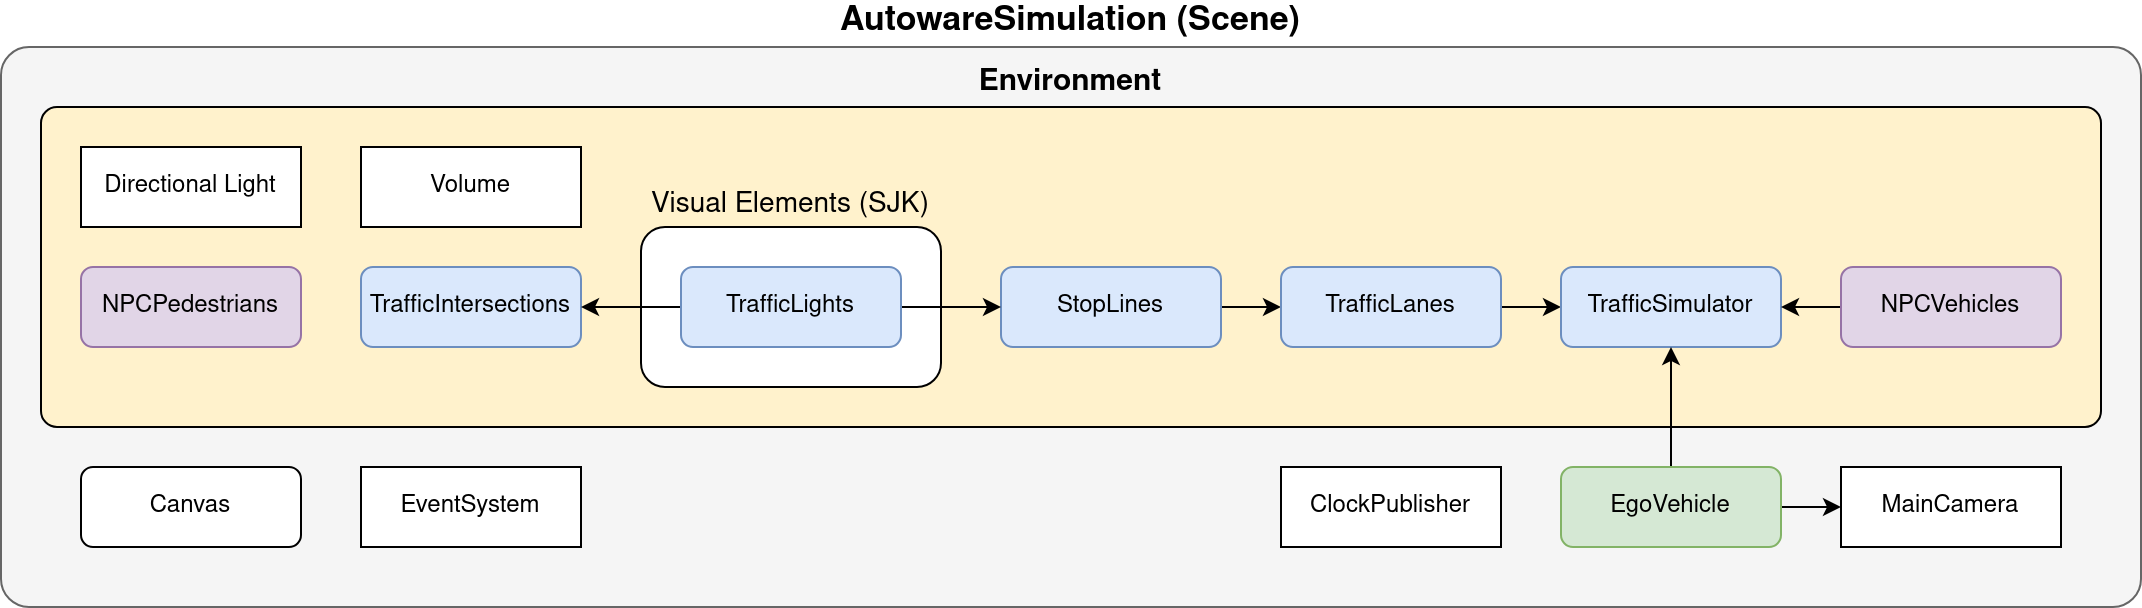
\includegraphics[width=1\linewidth]{figures/AWSIM_Architecture.png}
    \caption{معماری سطح بالای شبیه‌ساز \lr{AWSIM} \cite{AWSIM:Documentation}}
    \label{fig:AWSIM_Architecture}
\end{figure}

برای توصیف معماری \lr{AWSIM}، ابتدا باید به صحنه\LTRfootnote{\lr{Scene}} بازی اشاره کرد. این صحنه، تمام اشیاء موجود در شبیه‌سازی یک سناریو خاص و تنظیمات آن‌ها را شامل می‌شود. صحنه پیش‌فرض \lr{AWSIM} که برای کار با \lr{Autoware} توسعه یافته است، به نام \lr{AutowareSimulation} شناخته می‌شود.
در این صحنه می‌توان اجزاء اساسی مانند دوربین اصلی \lr{(MainCamera)}، انتشارکننده زمان \lr{(ClockPublisher)}، سیستم رویداد \lr{(EventSystem)} و کانواس \lr{(Canvas)} را مشاهده کرد. توضیحات دقیق در مورد صحنه و اجزای آن را می‌توان در صفحه توضیحات \lr{AWSIM} خواند\LTRfootnote{\url{https://tier4.github.io/AWSIM/ProjectGuide/Scenes/}}.
علاوه بر موارد ذکرشده، این صحنه دارای دو مؤلفه دیگر بسیار مهم و پیچیده به نام‌های محیط \lr{(Environment)} و خودروی خودران \lr{(EgoVehicle)} است. حال به توضیح هر کدام می‌پردازیم \cite{Autoware:Documentation}.

\subsection{مولفه محیط}
محیط، یک مؤلفه مهم است که تمام عناصر بصری\LTRfootnote{\lr{Visual Elements}} را که محیط را در صحنه شبیه‌سازی می‌کنند و همچنین کنترل بر روی آن‌ها فراهم می‌کنند را شامل می‌شود. این مؤلفه شامل دو زیر‌مؤلفه‌ی \lr{Light} و \lr{Volume} نیز می‌شود که به تأمین نور مناسب برای عناصر بصری و شبیه‌سازی شرایط آب و هوا می‌پردازند\LTRfootnote{\url{https://tier4.github.io/AWSIM/Components/Environment/AddNewEnvironment/AddEnvironment/\#create-an-environment-prefab}}.
علاوه بر عناصر بصری مانند ساختمان‌ها و برگ‌ها، این مؤلفه شامل کلیه ساختار مربوط به ترافیک نیز می‌شود. ترافیک شامل وسایل نقلیه غیرقابل کنترل \lr{(NPCVehicles)} می‌شود که توسط مولفه شبیه‌ساز ترافیک \lr{(TrafficSimulator)} در شبیه‌سازی ایجاد می‌شوند و از مولفه‌های مرتبط با ترافیک استفاده می‌کنند\LTRfootnote{\url{https://tier4.github.io/AWSIM/Components/Traffic/TrafficComponents/}}.
عناصر \lr{NPCPedestrians} نیز جزو مؤلفه‌های محیط به حساب می‌آیند، اما توسط مولفه شبیه‌ساز ترافیک کنترل نمی‌شوند. برای حرکت آن‌ها از کد‌هایی مخصوص استفاده می‌شود\LTRfootnote{\url{https://tier4.github.io/AWSIM/Components/Traffic/NPCs/Pedestrian/}}.
\begin{figure}[h!]
    \centering
    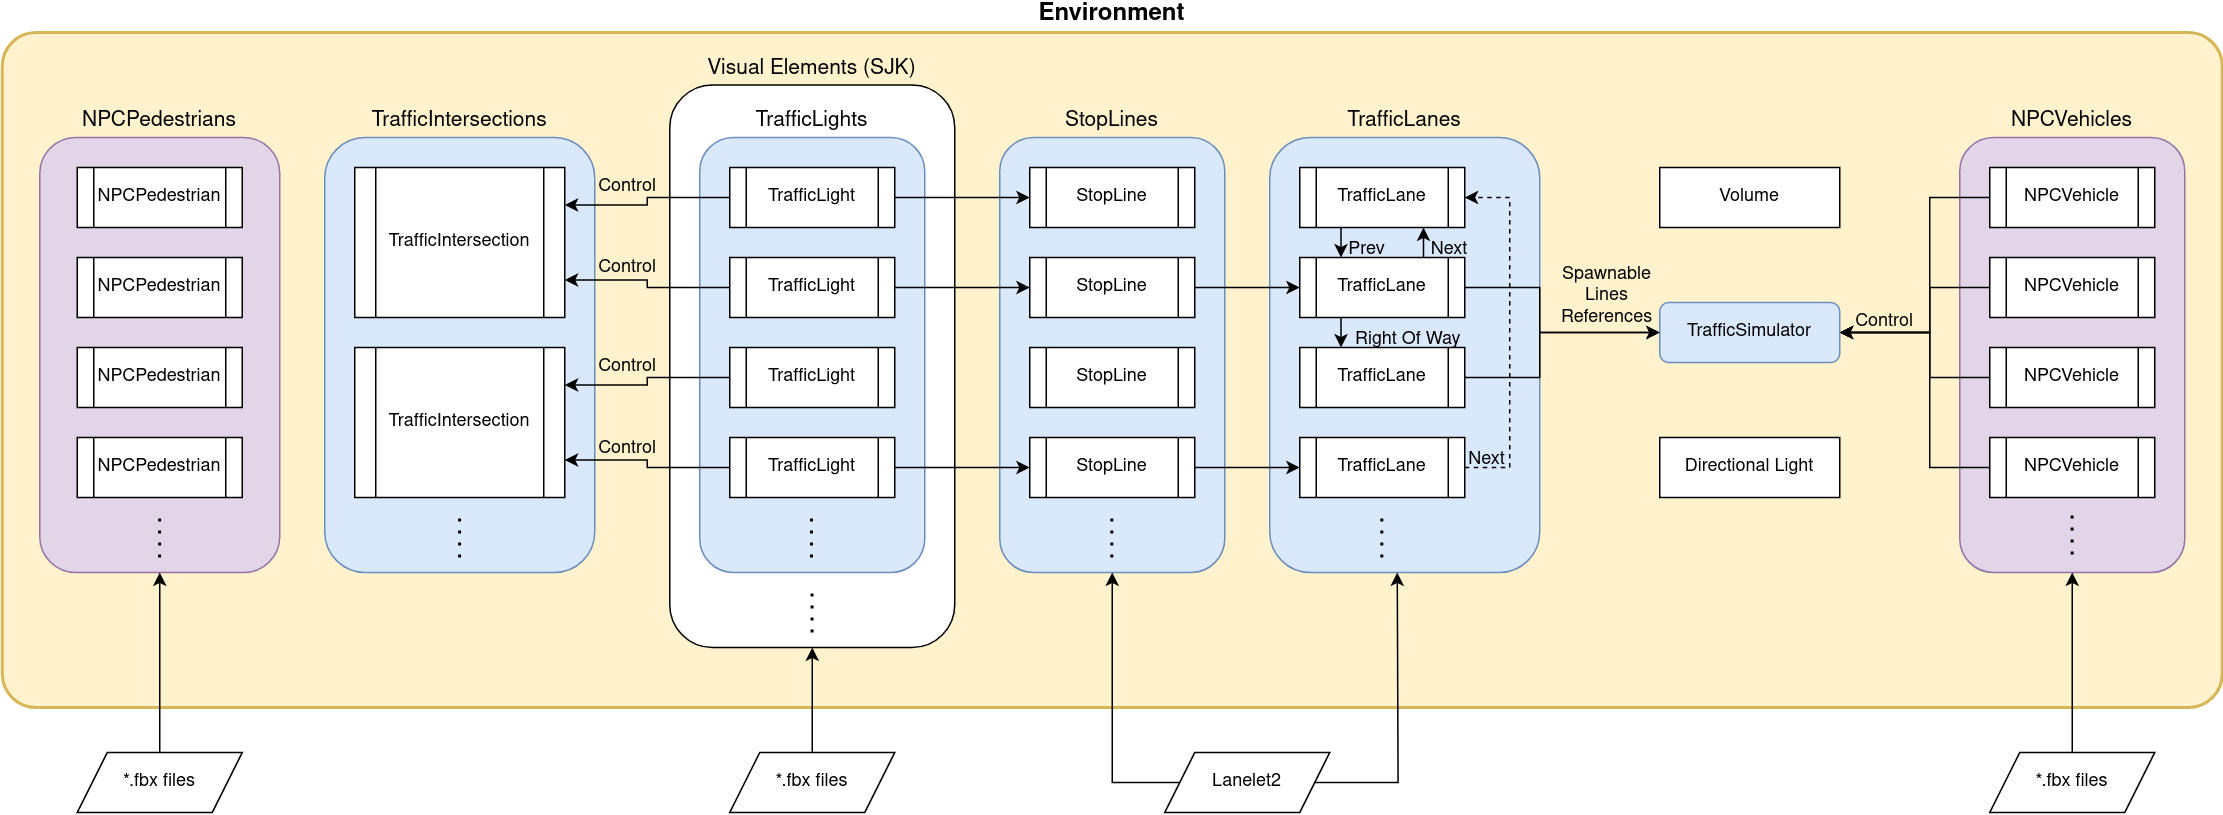
\includegraphics[width=1\linewidth]{figures/AWSIM_Environment_Architecture.png}
    \caption{معماری مولفه محیط شبیه‌ساز \lr{AWSIM} \cite{AWSIM:Documentation}}
    \label{fig:AWSIM_Environment_Architecture}
\end{figure}

\subsubsection{مولفه‌های ترافیک \lr{(Traffic)}}
مولفه‌های خطوط ترافیک \lr{(TrafficLanes)}  و خطوط ایست \lr{(StopLines)}،  عناصری هستند که از \lr{Lanelet2} (نرم‌افزار ساختن نقشه بُرداری) به محیط اضافه می‌شوند. خطوط ترافیک به گونه‌ای مراجعه متقابل\LTRfootnote{\lr{Cross-Reference}} دارند تا مسیرهایی را در محیط \lr{Unity} بر روی خطوط ترافیک ایجاد کنند. همچنین، هر خط ترافیک موجود در تقاطع\LTRfootnote{\lr{Intersection}}، شرایط خاصی برای اعطای حق تقدم دارد. مولفه شبیه‌ساز ترافیک، از مولفه خطوط ترافیک برای ایجاد \lr{NPCVehicles} و تضمین حرکت آن‌ها در امتداد این خطوط استفاده می‌کند. اگر برخی از خطوط ترافیک همچنان پیش از تقاطع به پایان برسند، دارای ارجاعی به خط ایست روبروی خود می‌باشند. هر خط ایست در تقاطع، دارای ارجاع به نزدیک‌ترین چراغ راهنمایی رانندگی \lr{(TrafficLight)} می‌باشد. چراغ‌های راهنمایی رانندگی به یکی از گروه‌های عناصر بصری تعلق دارند و رابطی برای کنترل عناصر بصری که منابع چراغ‌های ترافیکی (لامپ‌ها) را شبیه‌سازی می‌کنند، فراهم می‌کنند. یک مولفه تقاطع ترافیکی \lr{(TrafficIntersection)}، به تنهایی مسئول کنترل تمام چراغ‌های راهنمایی رانندگی در یک تقاطع است\LTRfootnote{\url{https://tier4.github.io/AWSIM/Components/Traffic/TrafficComponents/}} \cite{AWSIM:Documentation}.

\subsection{مولفه خودروی خودران}
\begin{figure}[h!]
    \centering
    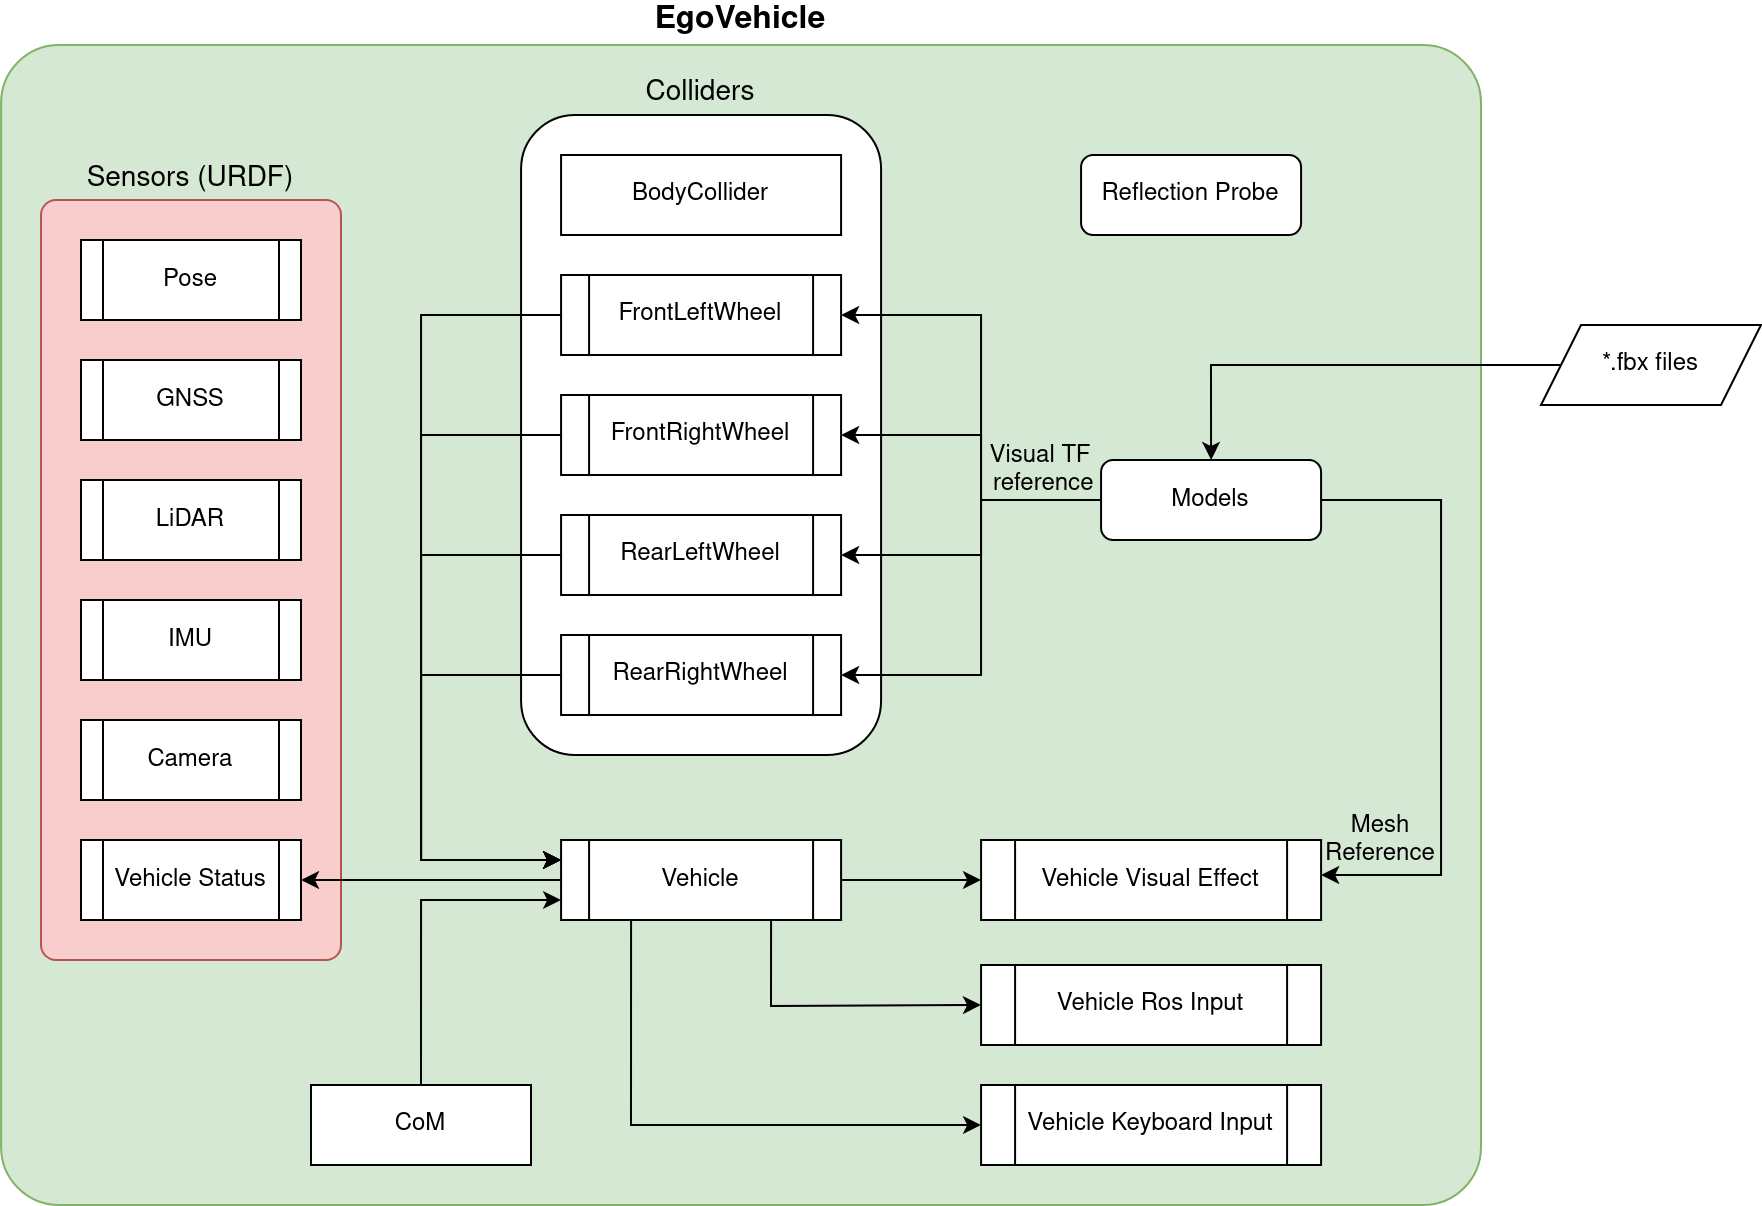
\includegraphics[width=1\linewidth]{figures/AWSIM_EgoVehicle_Architecture.png}
    \caption{معماری مولفه خودروی خودران شبیه‌ساز \lr{AWSIM} \cite{AWSIM:Documentation}}
    \label{fig:AWSIM_EgoVehicle_Architecture}
\end{figure}

مولفه خودروی خودران، یک مؤلفه مسئول برای شبیه‌سازی یک خودروی خودران، حین حرکت در صحنه است. این مولفه شامل موارد زیر می‌شود:
\begin{itemize}
    \item مولفه مدل‌ها \lr{(Models)} و \lr{Reflection Probe} که برای ظاهر دیداری ماشین هستند.
    \item مولفه برخورد‌ دهنده \lr{(Collider)}، که برخورد‌‌ها و قابلیت حرکت ماشین بر روی جاده‌ها را فراهم می‌کند.
    \item مولفه حسگر‌ها که داده‌های مرتبط با وضعیت خودرو در محیط، مانند موقعیت و سرعت آن را فراهم می‌کنند،
    \item مولفه وسیله نقلیه \lr{(Vehicle)}،‌ که دینامیک ماشین را شبیه‌سازی می‌کند و حرکت مولفه‌های چرخ \lr{(Wheel)} را کنترل می‌کند.
    \item مولفه‌های \lr{Vehicle Ros Input} و  \lr{ٰVehicle Keyboard Input} مرجعی به مولفه وسیله نقلیه دارند و دستورهای کنترلی را به آن می‌دهند.
    \item مولفه جلوه‌های بصری وسیله نقلیه ‌\lr{(Vehicle Visual Effects)}، که یک بستر را برای کنترل نورپردازی مولفه وسیله نقلیه، فراهم می‌کند.
\end{itemize}
توضیحات کامل این مولفه، در صفحه توضیحات شبیه‌ساز \lr{AWSIM}، آمده است\LTRfootnote{\url{https://tier4.github.io/AWSIM/Components/Vehicle/EgoVehicle/}}.

\subsection{شبیه‌ساز \lr{AWSIM} و ترکیب آن با \lr{Autoware}}
ترکیب \lr{Autoware} و \lr{AWSIM}، امکان بررسی درستی رفتار خودروی خودران را در سناریو‌های مختلف ترافیکی، فراهم می‌کند. 
\begin{figure}[h!]
    \centering
    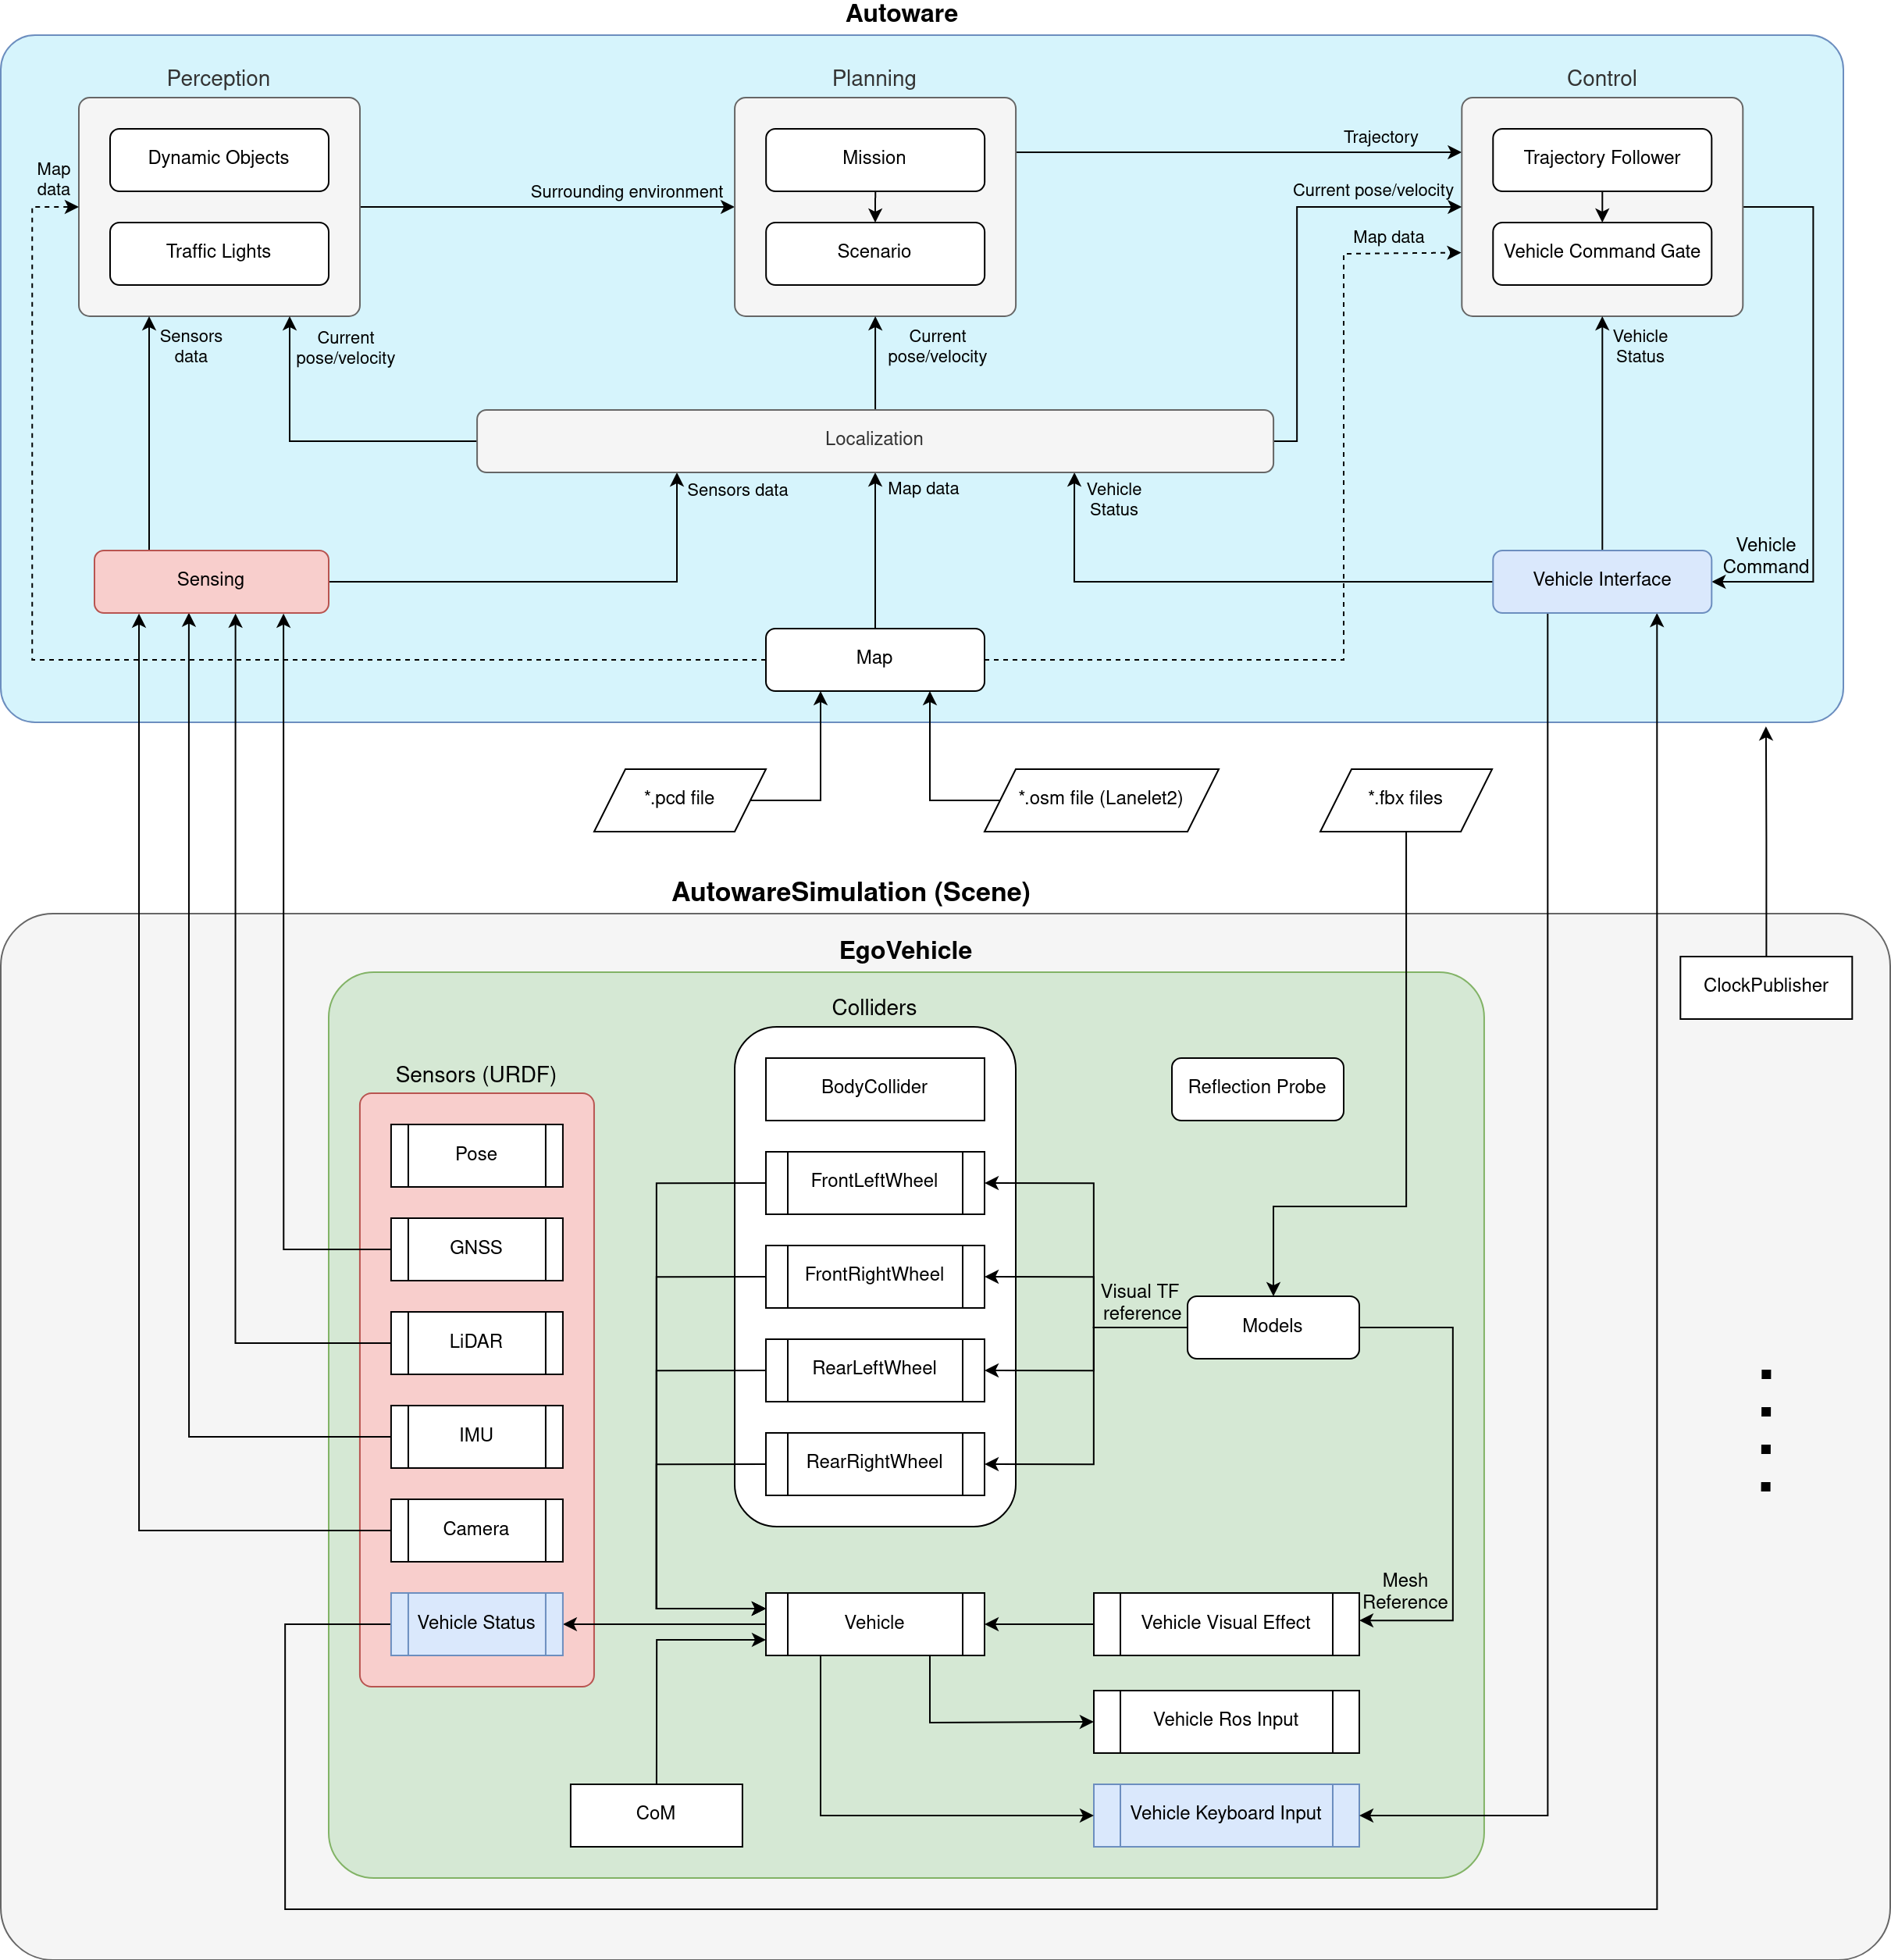
\includegraphics[width=0.85\linewidth]{figures/AWSIM_Autoware_Architecture.png}
    \caption{معماری ترکیب \lr{Autoware} و \lr{AWSIM} \cite{AWSIM:Documentation}}
    \label{fig:AWSIM_Autoware_Architecture}
\end{figure}
ترکیب \lr{AWSIM} با \lr{Autoware} به واسطه مولفه‌های بستر خودرو و احساس در معماری \lr{Autoware} امکان‌پذیر است. مولفه مسئول برای اطمینان از ارتباط با این مدول‌ها از سوی \lr{AWSIM}،  مولفه، \lr{EgoVehicle} است. این مولفه، به معماری \lr{Autoware} تطبیق یافته‌ و ارتباط بر اساس مباحث \lr{ROS2} را فراهم می‌کند. با این حال، یک اجزا مهم دیگر به نام انتشار‌کننده زمان وجود دارد که زمان شبیه‌سازی را برای \lr{Autoware} فراهم می‌کند و همچنین بر روی یک مبحث \lr{ROS2} منتشر می‌شود\LTRfootnote{\url{https://tier4.github.io/AWSIM/Components/ROS2/ROS2ForUnity/\#extension-scripts}}.

مؤلفه \lr{EgoVehicle} اطلاعات حال حاضر خودرو را از طریق یک اسکریپت درون مولفه وضعیت خودرو (\lr{Vehicle Status}) منتشر می‌کند. این اطلاعات به صورت بلادرنگ ارائه می‌شود و شامل مواردی نظیر: سرعت جاری، جهت گیری چرخ‌ها یا وضعیت جاری چراغ‌های خودرو است، که از سوی \lr{AWSIM} به‌دست می‌آیند و خروجی‌های آن هستند.

از سوی دیگر، مؤلفه \lr{Vehicle Ros Input}، مسئول ارائه مقادیر خروجی از \lr{Autoware} است. این مؤلفه در دستورات جاری مرتبط با شتاب دادن، دنده‌های گیربکس یا کنترل نورهای مشخص مشترک می‌شود.

اجرای دستورات دریافتی از طریق مؤلفه وسیله نقلیه امکان‌پذیر است، که تنظیم شتاب مناسب بر روی چرخ و کنترل عناصر بصری خودرو را انجام می‌دهد.

سایر داده‌های ارسالی از سوی \lr{AWSIM} به \lr{Autoware}، اطلاعات حسگرها هستند که اطلاعاتی در مورد وضعیت فعلی محیط اطراف و اطلاعات مورد نیاز برای تخمین دقیق موقعیت \lr{EgoVehicle} را فراهم می‌کند\LTRfootnote{\url{https://tier4.github.io/AWSIM/Introduction/CombinationWithAutoware/}} \cite{AWSIM:Documentation}.

\begin{figure}[h!]
    \centering
    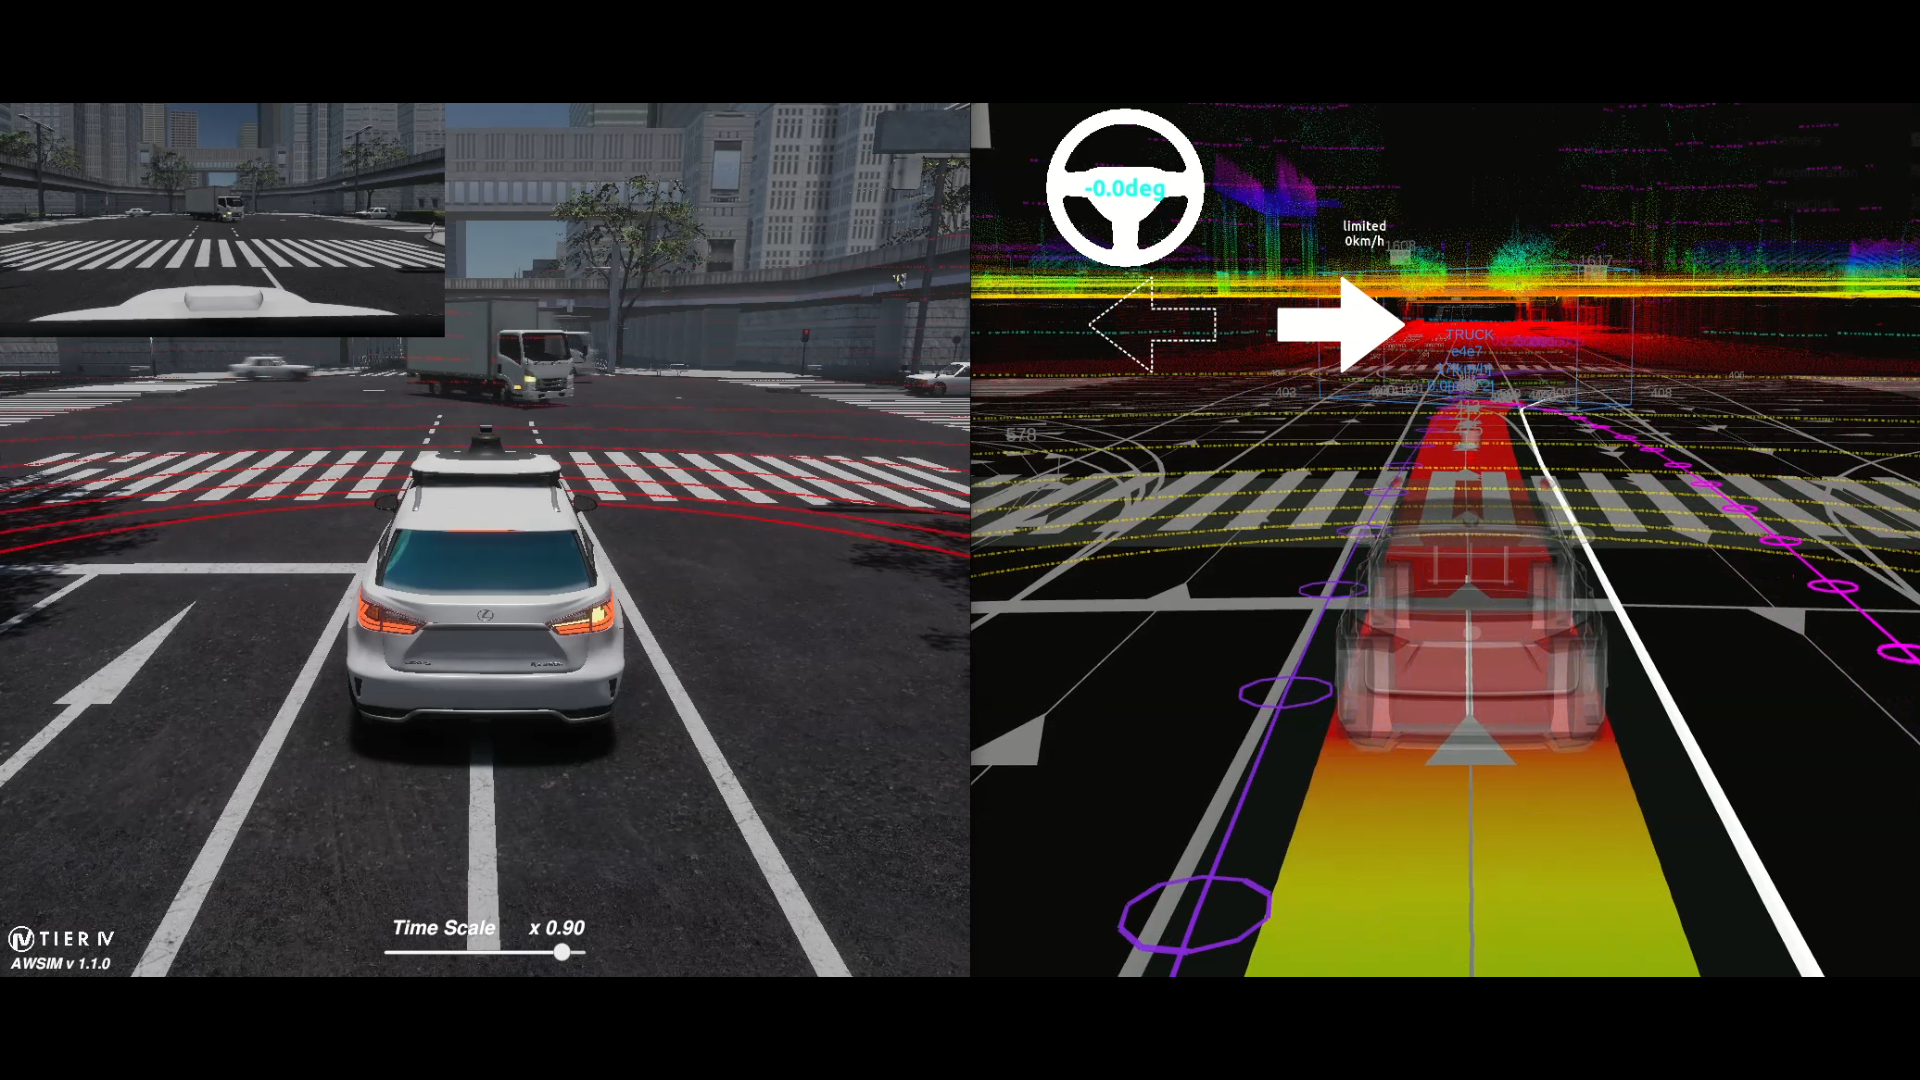
\includegraphics[width=0.95\linewidth]{figures/AWSIM_Autoware_Combination.png}
    \caption{تصویری از همکاری شبیه‌ساز \lr{AWSIM} (سمت چپ) و نرم‌افزار \lr{Autoware}} (سمت راست) \cite{AWSIM:Documentation}
    \label{fig:AWSIM_Autoware_Combination}
\end{figure}

\subsection{افزونه \lr{ROS2ForUnity}}
مدول \lr{Ros2ForUnity (R2FU)} یک راه‌حل ارتباطی است که به طور موثر، اتصالی بین موتور بازی‌سازی \lr{Unity} و بستر \lr{ROS2} ایجاد می‌کند و یک ادغام قوی را تشکیل می‌دهد. این مدول، برخلاف راه‌حل‌های دیگر، از ارتباط مستقیم استفاده می‌کند و به‌جای استفاده از پل ارتباطی، از پشته میان‌افزاری \lr{ROS2} (به ویژه کتابخانه کلاینت \lr{rcl} و لایه‌های پایین‌تر آن) استفاده می‌کند، که امکان اضافه کردن گره‌های \lr{ROS2} را به شبیه‌سازی‌های \lr{Unity} را فراهم می‌کند.

\lr{R2FU} در \lr{AWSIM}، به دلایل متعددی استفاده می‌شود. اول از همه‌ چیز، به علت ارائه ادغامی با عملکرد بالا بین \lr{Unity} و \lr{ROS2}، با بهبود توانایی انتقال و کاهش تأخیر نسبت به راه‌حل‌های پل ارتباطی، این مدول قابلیت‌های واقعی \lr{ROS2} را برای موجودیت‌های شبیه‌سازی در \lr{Unity} فراهم می‌کند، پیام‌های استاندارد و سفارشی\LTRfootnote{\lr{Custom}} را پشتیبانی می‌کند و انتزاعات\LTRfootnote{\lr{Abstractions}} و ابزارهای مفیدی را ارائه می‌دهد که همگی به عنوان یک عنصر \lr{Unity} تعبیه شده‌اند.

افرونه \lr{R2FU}، برخی از پیام‌های نرم‌افزارهای \lr{ROS2} و \lr{Autoware} را به صورت پیش‌فرض، پشتیبانی می‌کند که در \cref{tab:R2FU_Messages_Table} مشاهده می‌شوند:
\begin{table}[h!]
    \centering
    \caption{جدول پیام‌های پشتیبانی شده توسط \lr{R2FU} \cite{AWSIM:Documentation}}
    \begin{tabular}{|c|c|}
         \hline
         \textbf{بسته} & \textbf{پیام} \\
         \hline
         \multirow{5}{*}{\textbf{\lr{common\_interfaces}}} & \lr{std\_msgs} \\ & \lr{geometry\_msgs} \\ & \lr{sensor\_msgs} \\ &  \lr{nav\_msgs} \\ & \lr{diagnostic\_msgs} \\
         \hline
         \multirow{4}{*}{\textbf{\lr{rcl\_interfaces}}} & \lr{builtin\_interfaces} \\ & \lr{action\_msgs} \\ & \lr{rosgraph\_msgs} \\ &  \lr{test\_msgs} \\
         \hline
         \multirow{5}{*}{\textbf{\lr{autoware\_auto\_msgs}}} & \lr{autoware\_auto\_control\_msgs} \\ & \lr{autoware\_auto\_geometry\_msgs} \\ & \lr{autoware\_auto\_planning\_msgs} \\ &  \lr{autoware\_auto\_mapping\_msgs} \\ & \lr{autoware\_auto\_vehicle\_msgs} \\
         \hline
         \multirow{2}{*}{\textbf{\lr{tier4\_autoware\_msgs}}} & \lr{tier4\_control\_msgs} \\ & \lr{tier4\_vehicle\_msgs} \\
         \hline
         \multirow{2}{*}{\textbf{\lr{others}}} & \lr{tf2\_msgs} \\ & \lr{unique\_identifier\_msgs} \\
         \hline
    \end{tabular}
    \label{tab:R2FU_Messages_Table}
\end{table}
برای اینکه بسته پیامی سفارشی را بتوان در \lr{Unity} استفاده کرد، بایستی فایل‌های \lr{*.dll} و \lr{*.so} آن توسط \lr{R2FU} ساخته شوند\LTRfootnote{\url{https://tier4.github.io/AWSIM/Components/ROS2/ROS2ForUnity/}} \cite{AWSIM:Documentation}.

\section{موتور بازی \lr{Unity}}
\lr{Unity}، یک موتور بازی\LTRfootnote{\lr{Game Engine}} و سکو توسعه‌ی گسترده است که در صنایع بازی و رسانه‌های تعاملی بسیار محبوب است. این موتور بازی، به دلیل چند منظوره گرایی و دسترسی آسان شناخته شده است و به موتور انتخابی برای توسعه‌دهندگان تبدیل شده است، که قصد دارند محتوای گسترده‌ای از بازی‌های کامپیوتری تا برنامه‌های واقعیت افزوده و شبیه‌سازی‌ها را ایجاد کنند. \lr{Unity} سکو‌های مختلف را پشتیبانی می‌کند و این امکان را به توسعه‌دهندگان می‌دهد که پروژه‌های خود را بر روی دستگاه‌های مختلف مانند کامپیوتر شخصی، تلفن همراه، کنسول و حتی هدست‌های واقعیت مجازی/افزوده اجرا کنند. فروشگاه عناصر یونیتی دارای مجموعه‌ای بزرگ از منابع پیش‌ساخته، اسکریپت‌ها و ابزارها است که توسعه‌ی پروژه‌ها را ساده‌تر و سریع‌تر می‌کند، در حالی که سیستم اسکریپت‌نویسی بصری‌اش به نام "\lr{Bolt}" به افرادی که برنامه‌نویس نیستند اجازه می‌دهد تا رفتارها و تعامل‌های پیچیده‌ای را ایجاد کنند. اسکریپت‌های این موتور، با زبان برنامه‌نویسی \lr{C\#} نوشته می‌شوند.

\begin{figure}[h!]
    \centering
    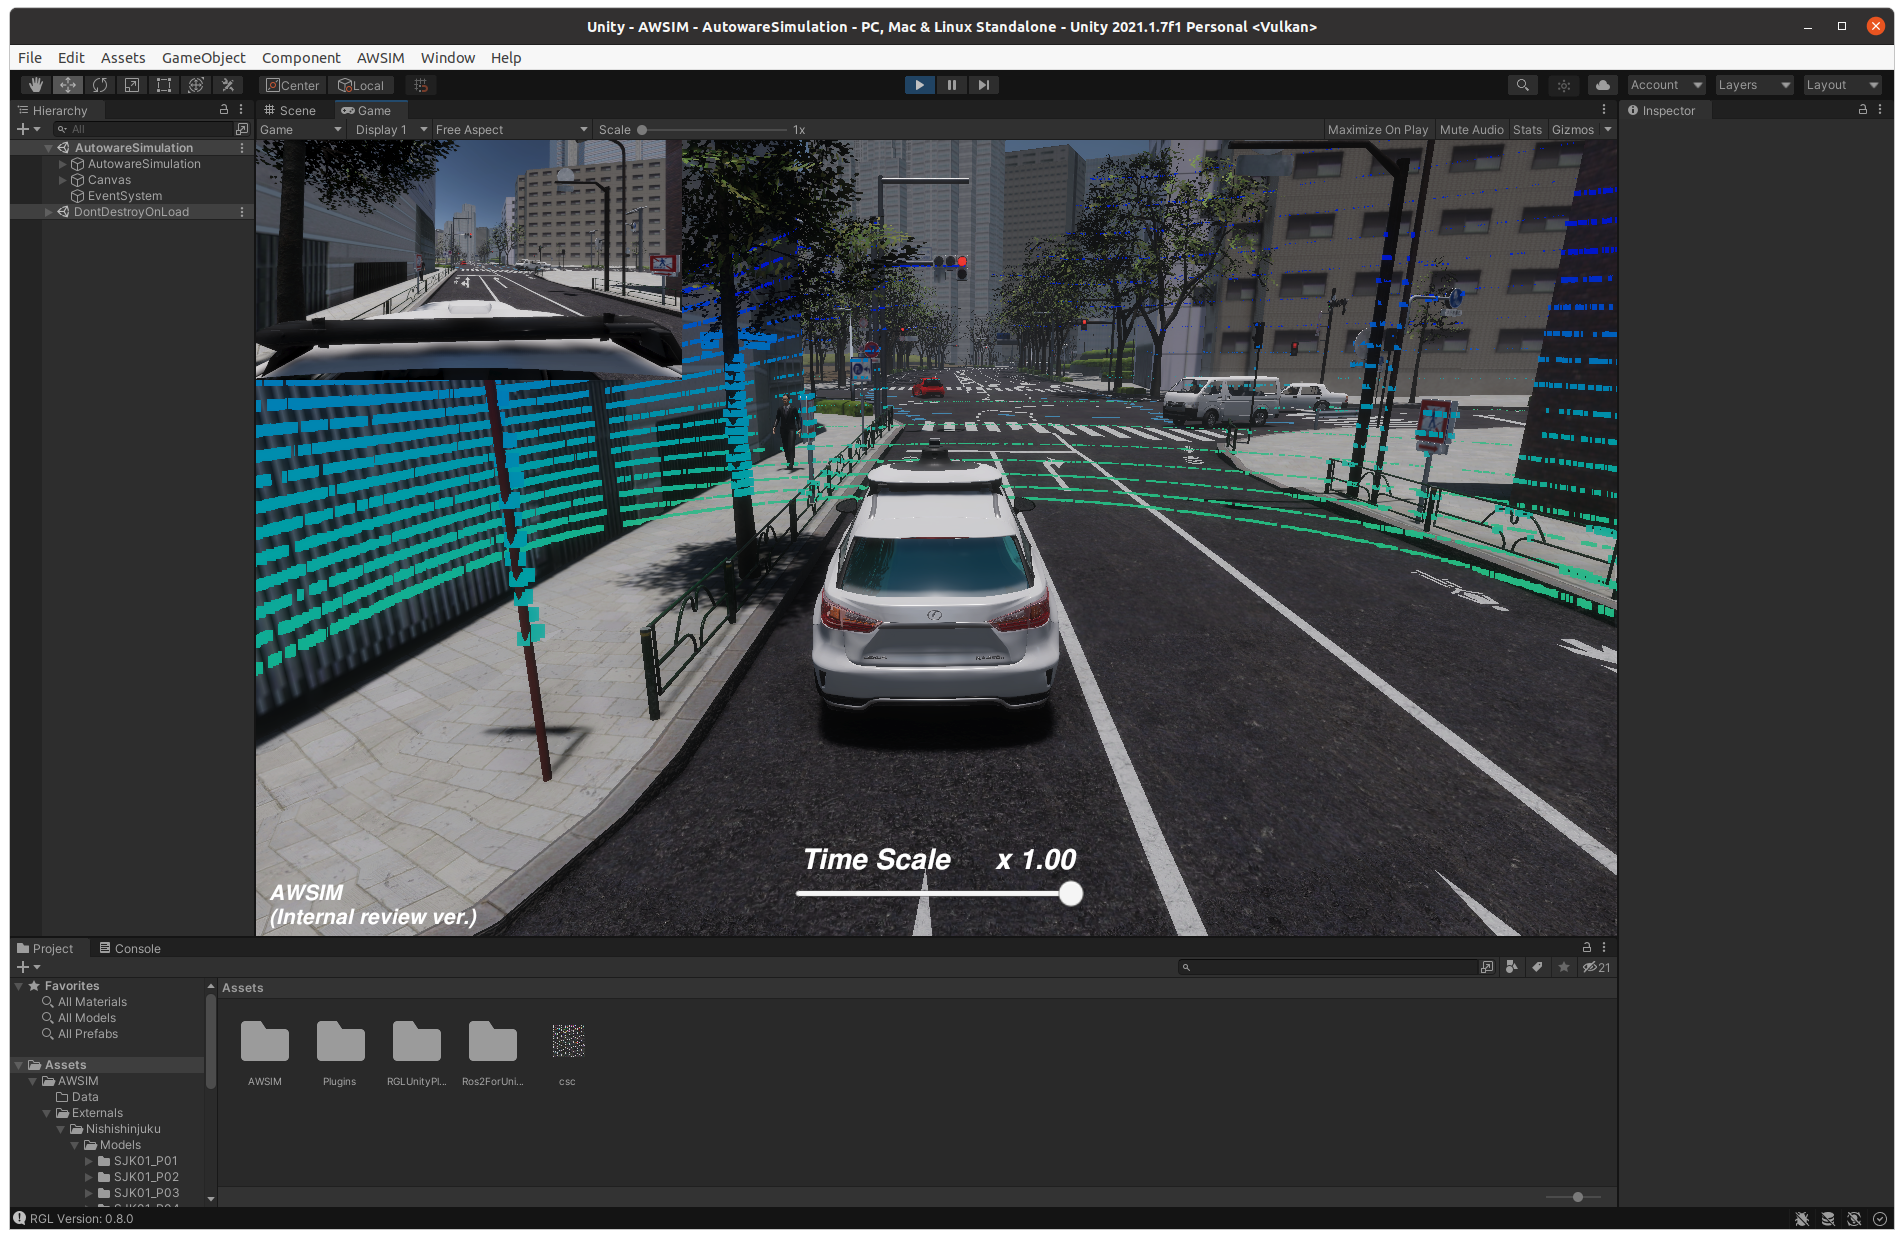
\includegraphics[width=1\linewidth]{figures/Unity_Workspace.png}
    \caption{شبیه‌ساز \lr{AWSIM} در بستر موتو بازی \lr{Unity} \cite{AWSIM:Documentation}}
    \label{fig:Unity_Workspace}
\end{figure}

یکی از ویژگی‌های برجسته‌ی \lr{Unity}، توانایی پردازش بلادرنگ آن است، که تجربیاتی با کیفیت بالای بصری و تعاملی را ارائه می‌دهد. این موتور امکان نورپردازی و سایه‌دهی پویا، شبیه‌سازی فیزیکی و پشتیبانی از گرافیک‌های دو‌بعدی و سه‌بعدی را فراهم می‌کند که همگی اساسی برای ایجاد جهان‌های غنی و شبیه‌سازی‌های واقع‌گرایانه هستند. به علاوه، رابط کاربری کاربر پسند این موتور، به جفت توسعه‌دهندگان مبتدی و حرفه‌ای این امکان را می‌دهد که پروتوتایپ‌سازی و تکرار سریع ایده‌های خود را به واقعیت تبدیل کنند. با جامعه‌ی پررونق توسعه‌دهندگان و مستندات جامع، یونیتی همچنان در حال تکامل است و خالقان را به اجرای ایده‌های خلاقانه خود ترغیب می‌کند و موقعیت برتری را به عنوان یکی از موتورهای اصلی صنعت بازی،‌برای خود تثبیت می‌کند\LTRfootnote{\url{https://unity.com/}}.

\section{ابزار \lr{Blender}}
\lr{Blender} یک ابزار قدرتمند و چندکاره در دنیای مدل‌سازی سه‌بعدی، انیمیشن و رندرینگ\LTRfootnote{\lr{Rendering}} است که به عنوان یک نرم‌افزار متن‌باز معرفی شده و در دنیای مدل‌سازی سه‌بعدی، انیمیشن و رندرینگ جایگاه ویژه‌ای دارد. این نرم‌افزار به خاطر داشتن مجموعه‌ای گسترده از امکانات معروف است، که از مدل‌سازی سه‌بعدی و نقاشی تا ریگینگ\LTRfootnote{\lr{Rigging}}، انیمیشن و حتی ویرایش ویدیویی می‌پردازد. رابط کاربری دوستانه \lr{Blender}، به همراه مجموعه گسترده ابزار و امکانات، آن را مناسب برای جفت مبتدیان و هنرمندان ماهر می‌کند. این نرم‌افزار به دلیل عملکرد قوی خود و همچنین به عنوان یک جایگزین مقرون به صرفه برای راه‌حل‌های نرم‌افزاری سه‌بعدی متعلق به شرکت‌های مختلف، شناخته شده است. این ابزار، برای کار روی انیمیشن‌های پیچیده شخصیتی، تصویرسازی‌های معماری یا اشیاء بازی، ‌\lr{Blender} مجموعه‌ای جامع از ابزارها را فراهم می‌کند.

\begin{figure}[h!]
    \centering
    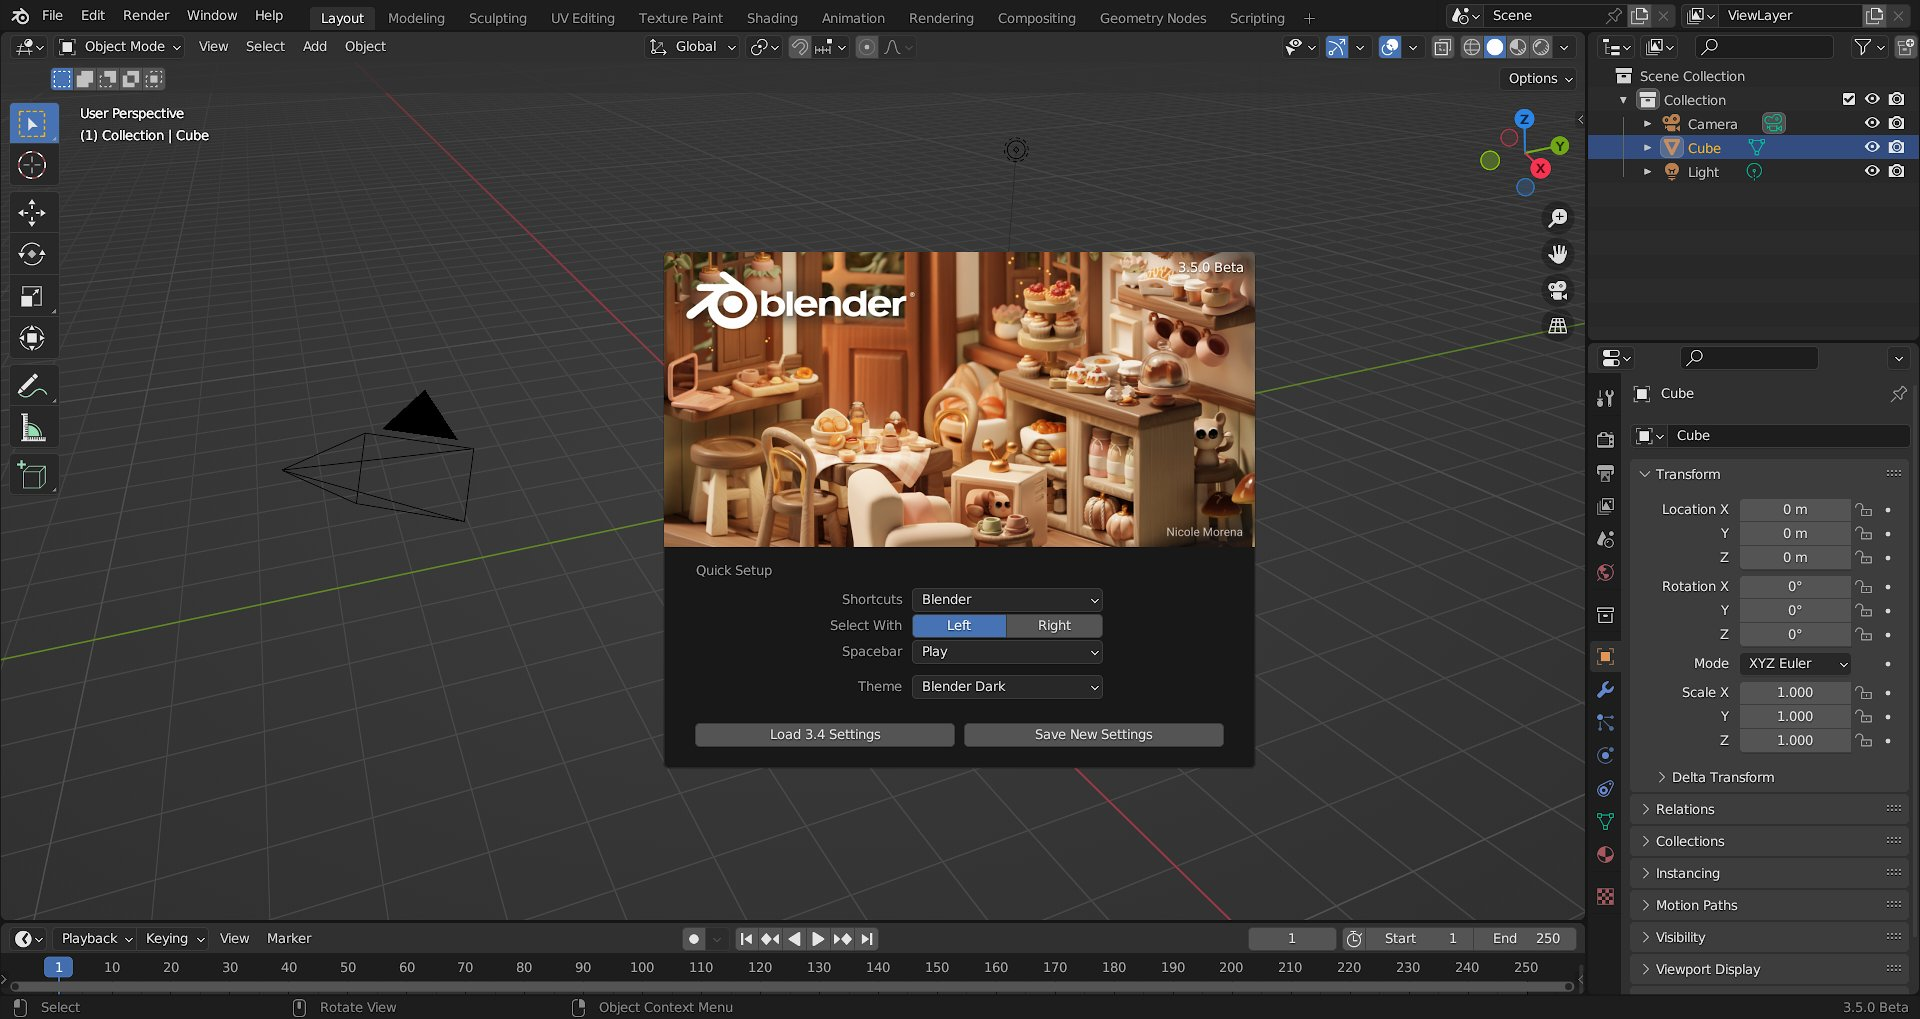
\includegraphics[width=1\linewidth]{figures/Blender.png}
    \caption{محیط ابزار \lr{Blender}}
    \label{fig:Blender}
\end{figure}

یکی از ویژگی‌های برجسته \lr{Blender}، ادغام آسان آن با \lr{Unity} است. یونیتی به طور پیش‌فرض، امکان وارد کردن فایل‌های \lr{Blender} را پشتیبانی می‌کند، که امکان بارگذاری مدل‌ها و انیمیشن‌های ایجاد شده در \lr{Blender} به طور مستقیم در پروژه‌های یونیتی را فراهم می‌کند. این سازگاری جریان کار را تسهیل می‌کند، زمان طی شده در فرآیند کار را کاهش می‌دهد و به هنرمندان اطمینان می‌دهد که بتوانند محتوای خود را در \lr{Blender} ایجاد کرده و آن را به سرعت در محیط \lr{Unity} مشاهده کنند. ترکیب قدرتمند مدل‌سازی سه‌بعدی و انیمیشن این ابزار، با ابزارهای توسعه بازی همانند \lr{Unity}، دنیایی از امکانات خلاقانه را ارائه می‌دهد و به توسعه‌دهندگان این امکان را می‌دهد تا محیط‌ها، شخصیت‌ها و اشیاء بازی را به راحتی طراحی و نمونه‌سازی کنند\LTRfootnote{\url{https://www.blender.org/}}.

\subsection{افزونه \lr{Blosm}}
\lr{Blosm}، که قبلاً به عنوان \lr{Blender-OSM} شناخته می‌شد، یک افزونه قدرتمند برای \lr{Blender} است که طراحی شده تا فرآیند وارد کردن داده‌ها و نقشه‌های جغرافیایی را ساده‌تر کند. با تنها چند کلیک، این افزونه دسترسی به مجموعه‌ای گسترده از منابع داده‌ای فراهم می‌کند، از جمله شهرهای سه‌بعدی گوگل، اطلاعات \lr{OpenStreetMap} و داده‌های پستی بلندی جهانی. این ابزار چند منظوره به کاربران این امکان را می‌دهد که به آسانی جزئیات جغرافیایی واقعی را به پروژه‌های \lr{Blender} خود وارد کنند. \lr{Blosm}، یک پروژه متن‌باز است. قابلیت‌های این افزونه بسیار قدرتمند است و به کاربران این امکان را می‌دهد تا انواع عناصر از جمله ساختمان‌ها، اشیاء آبی مانند رودخانه‌ها و دریاچه‌ها، مناطق گیاهی، جاده‌ها، مسیرها، راه‌آهن‌ها و داده‌های دقیق زمین با وضوح پوشش جهانی تقریباً 30 متر را وارد کنند\LTRfootnote{\url{https://github.com/vvoovv/blosm/wiki/Documentation}}.

\section{ابزار \lr{OpenStreetMap}}

ابزار طراحی نقشه‌برداری \lr{OpenStreetMap (OSM)}، یک پروژه مشترک و متن‌باز است که یک مخزن گسترده از داده‌های مکانی ارائه می‌دهد، شامل نقشه‌های دقیق و اطلاعات جغرافیایی که توسط داوطلبان از سراسر جهان تهیه می‌شود. این مشارکت‌ها مجموعه‌ای وسیع از ویژگی‌های جغرافیایی از جمله جاده‌ها، نمادها، شهرها و موارد دیگر را در بر می‌گیرد، که از مهم‌ترین منابع برای برنامه‌هایی مانند ناوبری، برنامه‌ریزی شهری، مدیریت بحران و خدمات مکانی مختلف هستند. مدل داده باز \lr{OSM}، کاربران را تشویق به ویرایش و بهبود نقشه‌ها می‌کند، تضمین می‌کند که داده‌های این پلتفرم به‌روز می‌شود و برای مجموعه‌ای گسترده از موارد کاربردی معتبر باقی می‌ماند.

\begin{figure}[h!]
    \centering
    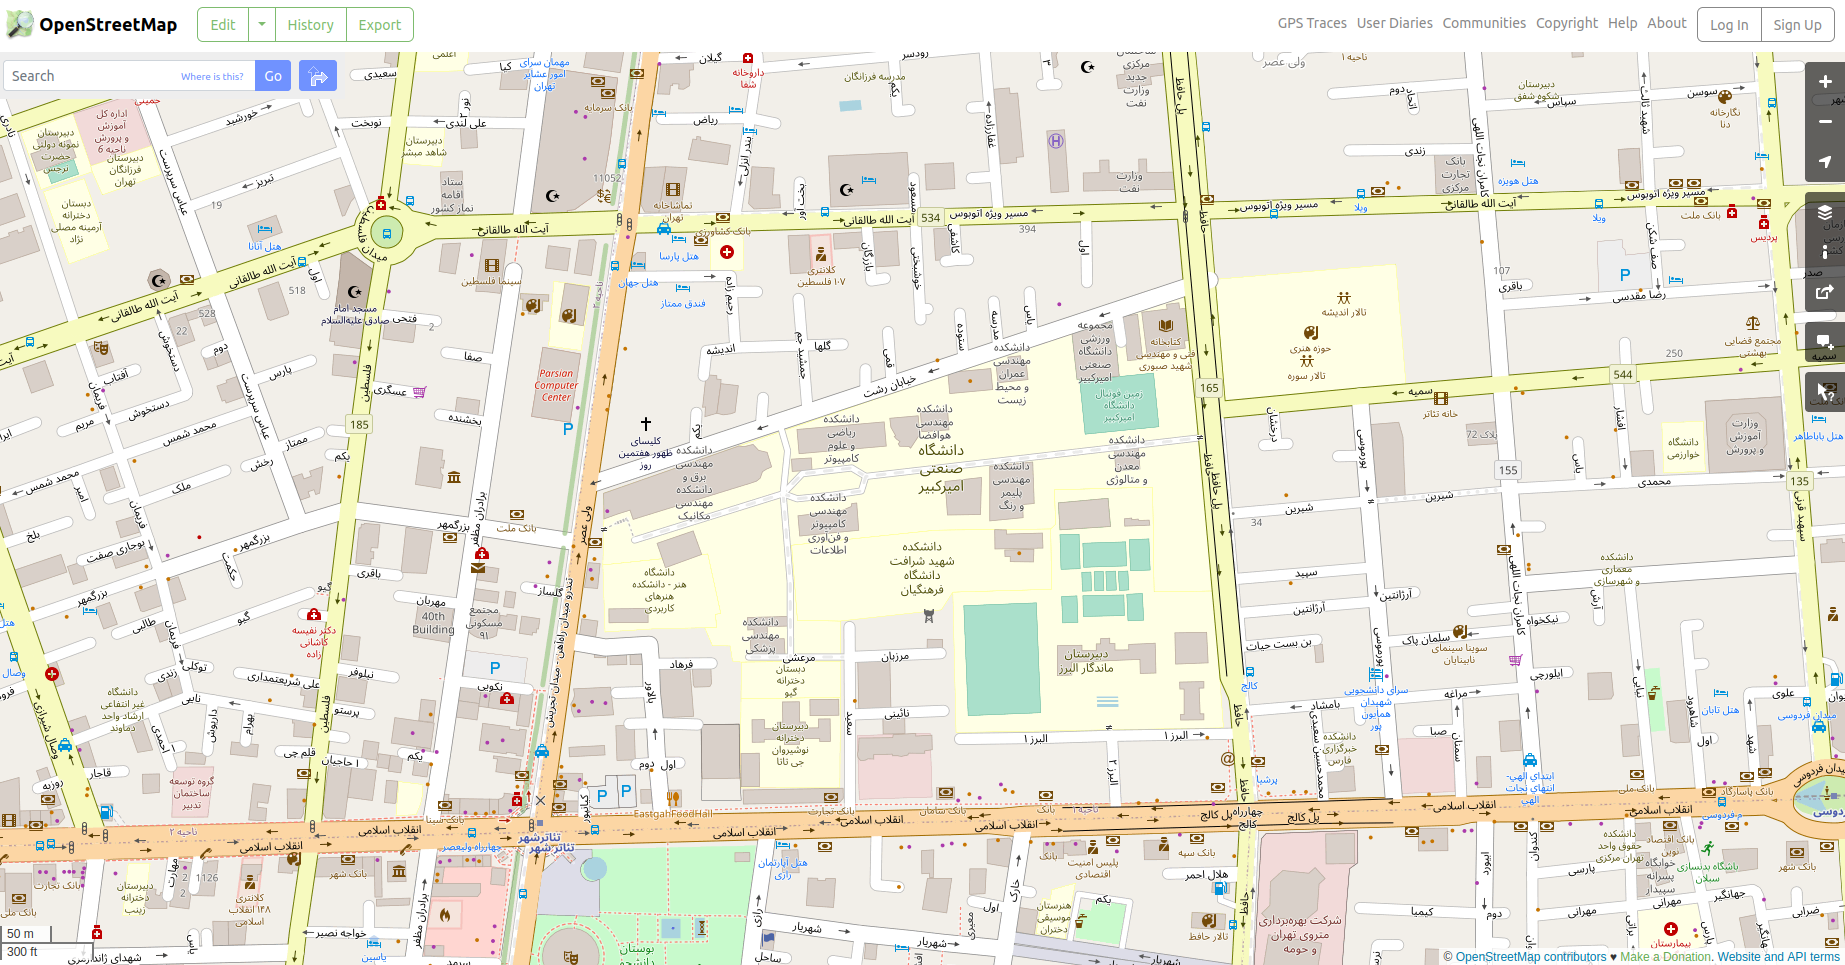
\includegraphics[width=1\linewidth]{figures/Amirkabir_OpenStreetMap.png}
    \caption{نقشه دانشگاه صنعتی امیرکبیر در ابزار \lr{OSM}}
    \label{fig:Amirkabir_OpenStreetMap}
\end{figure}

\section{کتابخانه \lr{OusterSDK}}
کتابخانه توسعه نرم‌افزار حسگرهای لایدار شرکت \lr{Ouster}، واسطه‌هایی را برای تعامل با سخت‌افزار حسگر و داده‌های حسگر ضبط‌شده که برای انجام آزمون‌ها، ارزیابی، و برنامه‌های غیرمرتبط با ایمنی، مناسب هستند را در زبان‌های پایتون و \lr{C++} فراهم می‌کند. کدهای مثال و مرجع برای عملیات معمول بر روی داده‌های حسگر در هر دو زبان نیز ارائه شده است. این کتابخانه، شامل واسط‌های برنامه‌نویسی برای:
\begin{enumerate}
    \item پرس‌‌وجوی تنظیمات حسگر و تنظیمات آنها
    \item ضبط و خواندن داده‌ها به فرمت \lr{.pcap}
    \item خواندن و بافرینگ داده‌های \lr{UDP} به صورت قابل اطمینان
    \item تبدیل داده‌های خام به تصاویر فاصله\LTRfootnote{\lr{Range}}، سیگنال، \LTRfootnote{\lr{Signal}}نور مادون قرمز نزدیک\LTRfootnote{\lr{Near-IR}}، انعکاس‌پذیری\LTRfootnote{\lr{Reflectivity}}
    \item  تبدیل اندازه‌گیری‌های کانال فاصله به مختصات کارتزین $(x, y, z)$
\end{enumerate}
علاوه بر این، این کتابخانه در زبان پایتون قابلیت‌های زیر را نیز دارد:
\begin{enumerate}
    \item دسترسی به فریم‌های داده‌های لایدار به عنوان داده‌های \lr{numpy}
    \item یک ابزار نمایشگر برای داده‌های ضبط شده‌ی \lr{.pcap} و حسگر لایدار \cite{OusterSDK:Documentation} (\cref{fig:OusterSDK_Visualizer})
\end{enumerate}

\begin{figure}[h!]
    \centering
    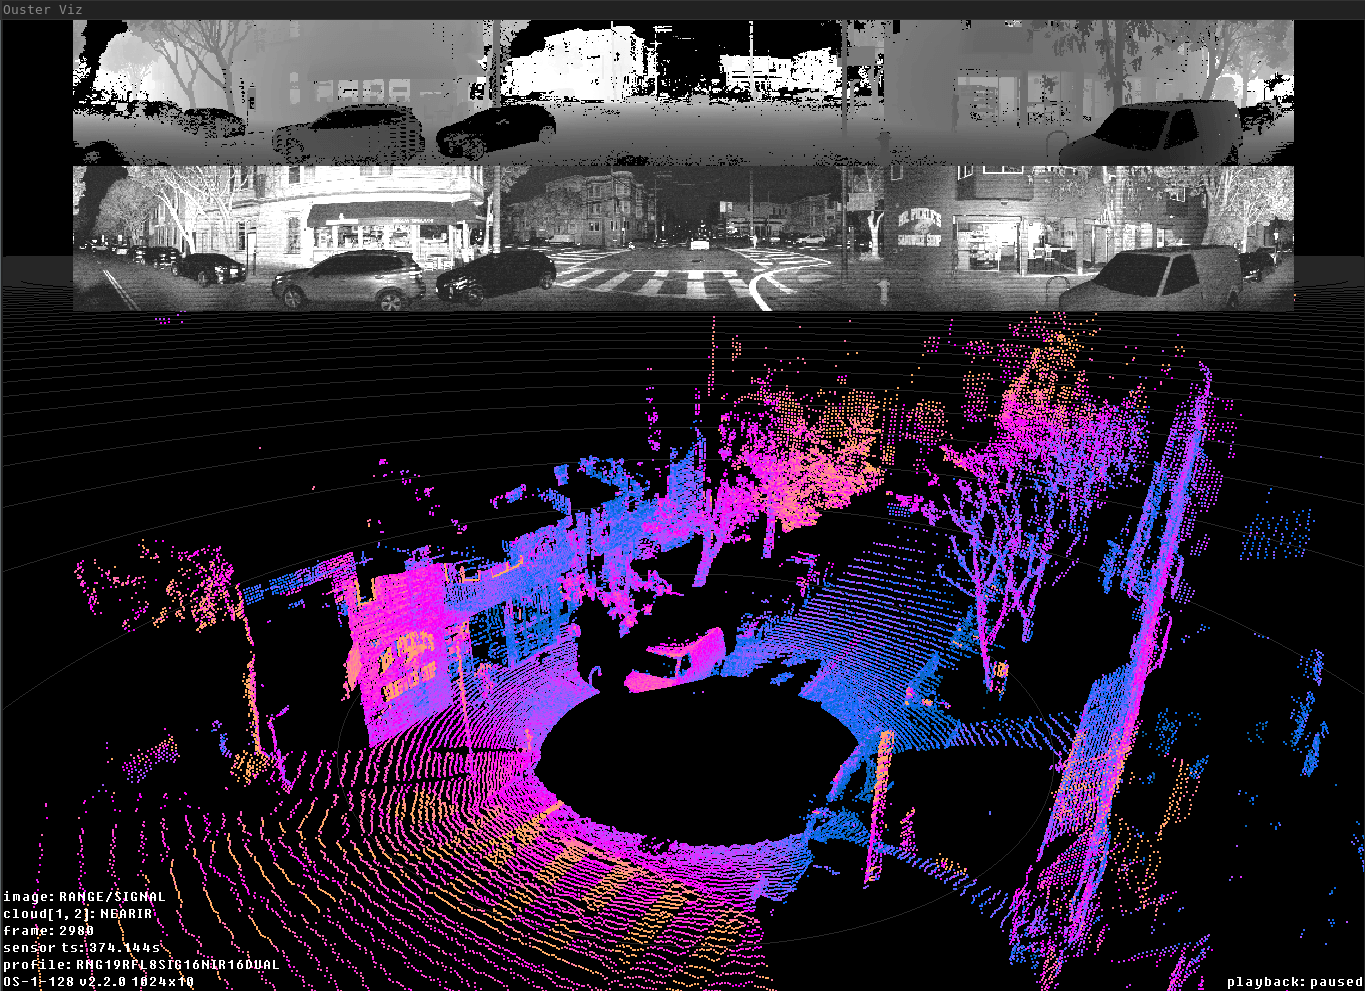
\includegraphics[width=1\linewidth]{figures/OusterSDK_Visualizer.png}
    \caption{ابزار نمایشگر کتابخانه \lr{OusterSDK} برای ابر نقاط \cite{OusterSDK:Documentation}}
    \label{fig:OusterSDK_Visualizer}
\end{figure}

\section{ابزار \lr{Ouster Studio}}
ابزار \lr{Ouster Studio} یک نرم‌افزار قدرتمند و کاربرپسند است که برای پردازش و نمایش داده‌های لایدار توسعه یافته است. با \lr{Ouster Studio}، شما می‌توانید به سرعت و سادگی داده‌های لایدار \lr{Ouster} را وارد کرده، تجزیه و تحلیل کرده و نمایش دهید. این نرم‌افزار برای ساده‌تر کردن فرآیند تنظیم و نمایش حسگرها ساخته شده و با کشف خودکار حسگر، امکان تشخیص و شناسایی حسگرهای متصل به یک شبکه یا سیستم را فراهم می‌کند. علاوه بر این، امکان پخش زنده، به کاربران این امکان را می‌دهد که داده‌های حسگر را به صورت بلادرنگ دریافت و پردازش کنند، که می‌تواند برای به دست آوردن بینش‌های فوری و امکان تصمیم‌گیری به موقع، مفید باشد. این نرم‌افزار به شما این امکان را می‌دهد که داده‌ها را به سرعت خود مرور و مطالعه کنید؛ همچنین امکان به اشتراک گذاری ضبط‌ داده‌های لایدار ضبط شده و شناسایی الگوها و روندهای آن را فراهم می‌کند، که ممکن است در داده‌های بلادرنگ به سرعت مشخص نشود.